\documentclass{report}
\usepackage[utf8]{inputenc}
\usepackage{algorithm}
\usepackage{algpseudocode}
\usepackage{paracol}
\usepackage{amsmath}
\usepackage{amssymb}
\usepackage{multirow}
\usepackage{bm}

\usepackage{setspace}
\onehalfspacing

\usepackage{geometry}
\geometry{margin=1.1in}



\setlength{\parindent}{0pt}
\setlength{\parskip}{1em}

\usepackage{amsmath,amsthm,amsfonts,amssymb,amscd, fancyhdr, color, comment, graphicx, environ}
\usepackage{float}
\usepackage{mathrsfs}
\usepackage{enumerate}
\usepackage[hidelinks]{hyperref}


\hypersetup{
    colorlinks=false,
    linkcolor=blue,
    filecolor=magenta,      
    urlcolor=blue,
    citecolor=black
}

\title{Diffusion-based Vocoding for Real-Time Text-To-Speech}
\author{Lukas Gardberg}
\date{\today}

\DeclareMathOperator*{\argmax}{\arg\!\max}
\DeclareMathOperator*{\argmin}{\arg\!\min}

% Description of sections available in https://www.overleaf.com/project/633ee853c4abcf21aea5ca84
\begin{document}

\maketitle

\newpage

\chapter*{Abstract}

The emergence of machine learning based text-to-speech systems have made fully automated customer service voice calls, spoken personal assistants, and the creation of synthetic voices seem well within reach. However, there are still many technical challenges with creating such a  system which can generate audio quickly and of high enough quality. One critical component of the typical text-to-speech pipeline is the vocoder, which is responsible for producing the final waveform in the process. This thesis investigates solving the vocoder problem using a statistical framework called \textit{diffusion}, which is used to teach a neural network to sequentially transform noise into recorded speech. Experiments are done by extending the framework with three different theoretical improvements, and evaluating a range of different diffusion-based vocoders which use these improvements with respect to inference speed and audio quality. In addition to this, a new variant of one such improvement is proposed, called a "variance schedule", which is shown to perform on par with previously adopted methods. Greater training stability is also achieved via methods inspired by diffusion models for image generation. The extensions of the framework are found to have a mostly positive effect on model performance, and audio is shown to be able to be generated at a quality equal to current state-of-the-art vocoders based on Generative Adversarial Networks, but not at the same speeds. Furthermore, we find that it is possible for a diffusion-based vocoder to achieve a 12 times speed up while retaining a comparable audio quality, and are convinced that further speed ups are possible. Inference for a real-time text-to-speech application is thought to be viable using a graphics processing unit, but not a central processing unit\footnote{For listening examples, see: lukasgardberg.github.io/thesis-examples}.

\newpage

\tableofcontents

\newpage

\chapter{Introduction}

% Ta evenutellt inspiration från hifi-gan introduction

In recent years, the amount which humans utilize software systems for communication has increased significantly. Ranging from the early beginnings of email, text messaging, and cellular calls, to modern voice and video chats through mobile applications. However, as these technologies have progressed, so has our ability to automate parts of the interaction. Be it pre-recorded messages, selecting an option on your keypad, or automatically generating responses to emails.

One such area of innovation is spoken conversation, where modern communication software strives to make the interaction personal by developing systems that are adaptable with regards to the human on the receiving end. Such a system needs to be able to understand the chosen medium, interpret what the human is communicating, and respond appropriately. This entails a level of natural language understanding as well as the ability to generate a natural sounding spoken response, and is an active research area.

Efforts have historically aimed to mimic the biological systems which give rise to speech in humans, either mechanically \cite{von1791mechanismus}, or through formant synthesis and vocal chord modelling \cite{fant1970acoustic}. Significant progress has also been made using rule- and expert-based systems which incorporate knowledge from experts (such as linguists) in order to achieve natural speech \cite{klatt1980software}. In addition to this, concatenative speech synthesis has also produced promising results, and is based on stitching together pre-recorded audio clips in order to obtain a target pronunciation. However, all of these methods exhibit several drawbacks, e.g. in the form of limited flexibility, heavy reliance on human knowledge, and varying naturalness of speech \cite{tan2021survey}.

%\textipa{ri:d}

In order to overcome these challenges the use of statistical parametric speech synthesis (SPSS) has grown, which aims to model the varying processes in speech using parameterized models and large amounts of data. This approach is usually divided up into three steps: text analysis, parameter prediction (acoustic model), and synthesis (vocoder), as shown in Figure \ref{fig:TTS}. The first step involves processing the text to be spoken, which includes e.g. normalization, segmentation, and phoneme conversion, which gives more detail to the pronunciation of the text. Secondly an acoustic model is tasked with generating computer processable acoustic features, which can be seen as a compact representation of the characteristics of the audio. Lastly a vocoder model generates audio (e.g. an audio file) based on prior acoustic features \cite{zen2009statistical, tan2021survey}. 
% Image adopted from \cite{tan2021survey}.
\begin{figure}[H]
    \centering
    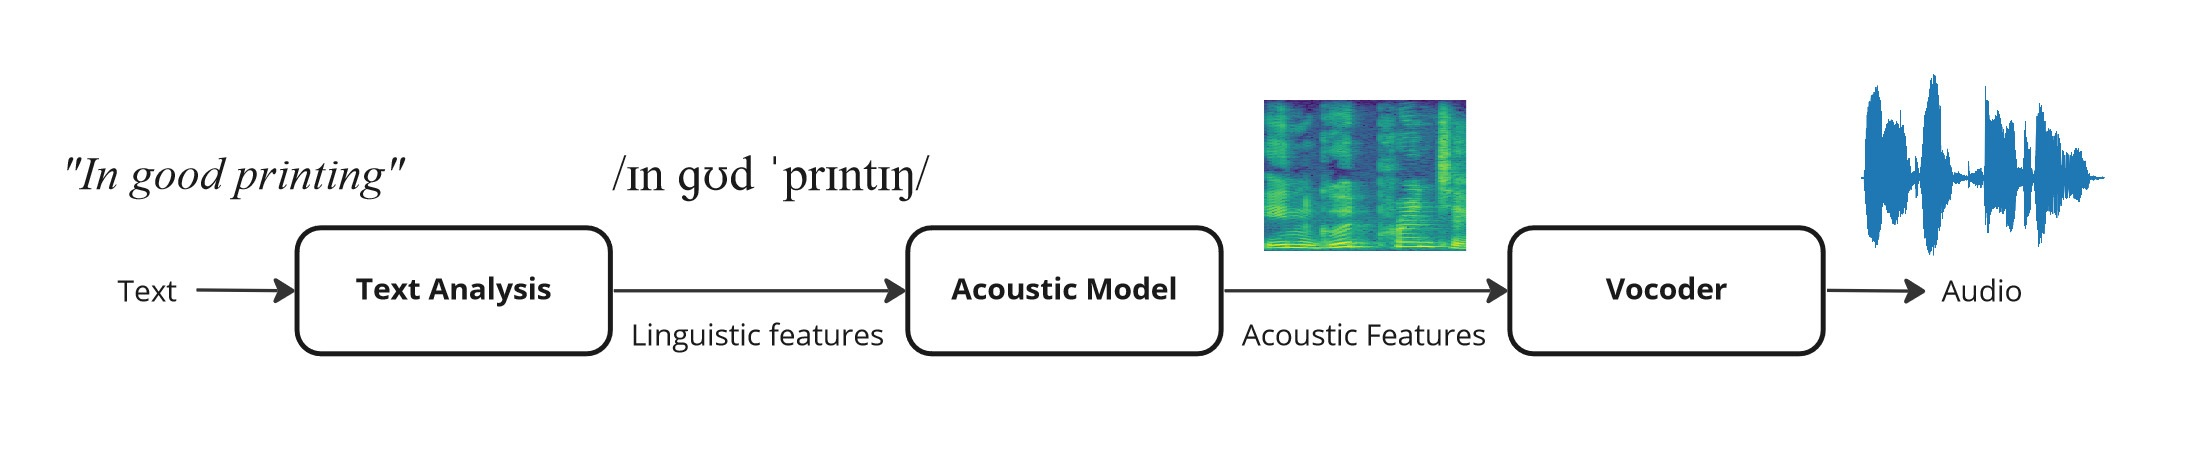
\includegraphics[scale=0.28]{images/TTS.jpg}
    \caption{\onehalfspacing Schematic overview of common text-to-speech components. The three blocks are typical intermediate steps, where an example of intermediate representations are shown above. The input text which speech is to be generated for is first analyzed to produce linguistic features. The example shows International Phonetic Alphabet (IPA) Symbols generated for the text \textit{"In good printing"}. These are then fed into an acoustic model outputting acoustic features, in this case a mel spectrogram. Lastly the acoustic features are converted into audio using a vocoder model.}
    \label{fig:TTS}
\end{figure}
Many of these ideas persisted in tandem with the rise of deep learning and the utilization of increased computational power. Neural networks have thus successfully been incorporated into all stages of SPSS \cite{ze2013statistical, arik2017deep}, and research has since moved towards a fuller end-to-end approach \cite{oord2016wavenet} which has seen great success in several other areas  \cite{krizhevsky2017imagenet, bojarski2016end, zhou2018voxelnet}. This has popularized the term \textit{neural text-to-speech}, where "end-to-end" refers to the task of generating speech directly from text, using no direct intermediate representations.

The recent rise of text-to-speech technologies is also of great interest to companies which handle  customer service interactions. One such company is Sinch, which this thesis is done in collaboration with. Sinch has a number of products which enable automated and personalized customer service, both through text and audio. The main appeal of voice driven customer service is that it can provide a more personal experience for the customer, as well as allow access to such services to a wider range of users in a more cost effective way. However, there are still many technical challenges with creating such a system, e.g. generating audio at at high speeds and of high enough quality.

This thesis focuses on the last step of the process, the \textit{vocoder}, and the challenge of creating high-quality audio using prior acoustic features. Special weight is put on \textit{diffusion-based} vocoders, and the aspects which currently limit such models from generating audio quickly.

\section{Previous Work}
The first vocoder based on neural networks is WaveNet which was proposed in 2016 \cite{oord2016wavenet}. Contrary to spectrograms it uses linguistic features directly as inputs in order to generate audio on the sample level. It is also autoregressive, meaning that each sample is conditioned on all previous ones, and that audio therefore is generated in a circular fashion by feeding in past outputs to the input. The backbone of WaveNet is the 1-D causal convolution layer, which provides learnable filters applied only on past samples relative to the current one. In addition to this, dilation is also leveraged in order to provide the filters with a wider receptive field and achieve greater efficiency. It is worth noting that one of the main drawbacks of WaveNet and similar autoregressive models is that waveform generation is not parallelizable, therefore resulting in a longer inference time via the inherent sequential nature. Several efforts have been made in order to reduce that time, for example through pruning or caching \cite{kalchbrenner2018efficient, paine2016fast}.

Later progress involved developing a fuller end-to-end sequence-to-sequence approach with Tacotron \cite{wang2017tacotron} and Tacotron 2 \cite{shen2018natural}. The proposed encoder in the first version addressed the limitations of using complex linguistic features, and instead aimed for a transformer-based model which produces mel spectrograms from character sequences. The vocoder part involved simple Griffin-Lim reconstruction, and was later improved in the second iteration. The improvement consisted of replacing the non-parametric vocoder with a WaveNet-based neural network which could be trained separately to the encoder to produce audio from mel spectrograms.

Following the advancement of using a neural network-based vocoder, several different directions have been taken. One of the main problems addressed is creating a non auto-regressive model, and speeding up inference through parallelizable architectures. One such family of models used as vocoders are \textit{flow-based} models. These utilize a normalizing flow which iteratively transforms a simple distribution into a complex one (i.e. the distribution of speech data) using a series of invertible mappings, and can thus achieve an approximation of a target posterior distribution \cite{rezende2015variational}. For example, WaveGlow \cite{prenger2019waveglow} is a flow-based vocoder which combines progress from Glow \cite{kingma2018glow} and WaveNet to non-autoregressively generate audio above 16kHz faster than real-time. 
%Interestingly, there are several similarities with denoising diffusion probabilistic models. Most notable is the iterative nature of the computations, and the idea of starting with a simple distribution, such as a unit Gaussian and sequentially obtaining a more complicated one.

In addition to this, generative adversarial networks (GANs) have also been utilized as vocoders \cite{goodfellow2020generative}. The principle behind a GAN is to jointly train a generator network to generate samples from noise, and a discriminator network to determine if a candidate sample is real or synthesized. Examples include WaveGAN \cite{donahue2018adversarial} which relies on a deep convolutional neural network as the generator, and improvements such as GAN-TTS \cite{binkowski2019high}, and HiFi-GAN \cite{kong2020hifi} which leverage techniques such as multiple discriminators and augmented loss functions. Such models are able to generate high fidelity audio effectively using only a single forward pass, but have been shown experimentally to be difficult to train (e.g. mode collapse) and are not able to produce likelihood estimates as a consequence of the architecture. However, they are widely considered to be the state-of-the-art in terms of inference speed.

The main model considered in this thesis is DiffWave \cite{kong2020diffwave}, which is the first diffusion-based vocoder, characterized by it's audio-specific architecture and conditioning on spectrograms generated by an acoustic model. The model is decribed in further detail in section \ref{sec:diffvoc}.

\section{Problem statement} \label{sec:statement}

The goal of this thesis is to explore the usage of denoising diffusion probablilistic models as vocoders, what aspects are favorable or limiting in real-time applications, and how they compare to other current machine learning-based models for speech generation. Here "real-time" refers to a system which can generate speech at approximately the same rate which humans speak. From the model's perspective we will consider this to correspond to the ability to generate an audio clip in less time than its duration, which is necessary for a text-to-speech system to be usable without too much delay. To achieve this, the aim is to answer the following questions:

\begin{itemize}
    \item How does inference speed and generated audio quality compare to a GAN-based vocoder?
    \item How do the following aspects affect inference speed and audio quality?
    \begin{itemize}
        \item Variance schedule
        \item Time-step importance sampling
        \item Noise prior
    \end{itemize}
    \item How does a vocoder trained on audio from one speaker generalize to another?
    \item Can such a model generate audio faster than real-time?
\end{itemize}

\textit{Inference} is here defined in the machine learning sense, which corresponds to the process of performing prediction on new data, i.e. generating audio from spectrograms. The inference speed therefore refers to how quickly the model can perform prediction.

\newpage
\chapter{Theory}

This section introduces the major theoretical building blocks needed to understand diffusion models, as well as tools and techniques related to the vocoder problem. The processing and analysis of audio signals is covered, including the three different waveform-, spectrogram-, and mel spectrogram-representations. In addition to this, a brief introduction to machine learning and learning algorithms is given in order to provide context for the modelling and optimization methods used. Lastly the diffusion framework is presented along with current limitations and challenges, as well as a discussion on suitable evaluation methods for generative models for audio.

\section{Sound \& Signals} \label{sec:sounds}

The natural representation of a sound, and what our human ears have evolved to perceive, is a repetitive increase and decrease in air pressure in the form of an acoustic wave. The source of a wave can for example be a vibrating membrane whose movement sets air into motion, such as our vocal cords. Each sound possesses a certain \textit{frequency} representing how many times the acoustic wave compresses and de-compresses (oscillates) per unit of time, and is measured in Hertz (Hz). Humans have evolved to perceive sounds with a frequency between 20 Hz and 20 kHz, where sounds outside of this range are inaudible to us. Sound is most commonly recorded via a microphone in which a fixture is displaced by the propagating wave. The component inside the microphone is configured to induce an electrical signal representing the movement of the air.

In order to represent such an analog signal digitally, its value (the amount of voltage or current) is measured at a certain rate, i.e. \textit{sampled}, where the discrete measurements are represented using quantized amplitude values such as floating point units. The rate at which the signal is measured is called the \textit{sample rate} $f_s$ (Hz). As a consequence of the Nyquist-Shannon sampling theorem a digital signal can only represent an analog signal without distortion (aliasing) if it is sampled with a sample rate at least double the frequency of the highest frequency in the analog signal. For example, a signal sampled at 44 100 Hz can at most adequately represent an analog signal of 22 050 Hz, making it an appropriate sample rate for human hearing. If distortions such as noise or other unwanted sounds end up in an audio signal they are often times called \textit{artefacts}.

Mathematically it is possible to represent an audio signal in several ways. One form suitable for theoretical analysis is to define it as a function $x: \mathbb{R} \rightarrow \mathbb{R}$, where $x(t)$ represents its amplitude at a real valued time-point $t \in \mathbb{R}$. However, in practice measured signals are not defined at infinitely many points, but are rather of limited size as a consequence of the time interval over which they were sampled being finite. We define such a real-word signal as a \textit{vector} $\bm{x} = [x[0], \, \dots, \, x[L-1]]^{\text{T}} \in \mathbb{R}^{L}$ which consists of $L$ real-valued amplitude samples indexed from $0$.

\subsection{The Short-Time Fourier Transform} \label{sec:stft}

For the task of analyzing the frequency contents of signals such as audio, the \textit{Fourier Transform} is a common and useful tool. Given a signal $x: \mathbb{R} \to \mathbb{R}$ its transform $\hat{x}: \mathbb{R} \to \mathbb{C}$ is defined as
\begin{equation}
\label{eq:fouriert}
    \hat{x}(f) = \int_{-\infty}^{\infty} x(t) e^{-i 2\pi f t} \, dt,
\end{equation}
for a specific frequency $f\in\mathbb{R}$. The resulting function $\hat{x}$ provides amplitude and phase information of each frequency contained in $x$ in the form of the absolute value and the argument of the resulting complex number. Intuitively the Fourier Transform can be interpreted as a measure of how correlated a signal is with a sinusoid of frequency $f$. Once $\hat{x}$ has been obtained, it is also possible to perform an inverse transform
\begin{equation}
    x(t) = \int_{-\infty}^{\infty} \hat{x}(f) e^{i 2\pi f t} \, df
\end{equation}
in order to recover the original signal $x$ under certain conditions.

As earlier described, signals are often represented as sampled values at discrete time points in contrast to a real valued function. The respective transform for a discrete-time signal $\bm{x}=\left[ x[0], x[1], \dots , x[L-1] \right]^{\text{T}}$ is the \textit{Discrete Fourier transform} (DFT), which is defined as
\begin{equation}
    \hat{x}[k] = \sum_{n=0}^{L-1} x[n] e^{-i \frac{2\pi}{L}k n},
\end{equation}
resulting in a new complex valued vector $\bm{\hat{x}} = [\hat{x}[0],\dots, \hat{x}[L-1]]^{\text{T}}$ where $\bm{\hat{x}}\in \mathbb{C}^{L}$. Worth noting is that both these transforms analyze the complete signal all at once which yields a static spectrum, and can thus be ill suited for signals whose frequency content change over time. An example of such a changing signal is recorded speech, where the pronunciation of different vowels and consonants in the form of sustained and plosive sounds result in a dynamic frequency distribution.

In order to account for this variability the signal can instead be analyzed at several overlapping individual segments. This is done by \textit{windowing} the signal with a window function $w$ which is zero outside of a set width. In practice this function is represented as a vector $\bm{w}=[w[0],\dots, w[l-1]] \in \mathbb{R}^l$ typically of length $l<L$. The resulting transform of such a windowed signal gives a representation of the frequency content of that particular segment, allowing several such windowed transforms to be combined into a time-dependent frequency distribution. This process is performed using the \textit{Short-Time Fourier Transform} (STFT), which for a signal $\bm{x}$ and window function $\bm{w}$ is defined as
\begin{equation} \label{eq:spec}
    \text{STFT}\left\{ \bm{x} \right\}(k, m) = Y[k, m] = \sum_{n=0}^{L-1} x[n]w[n-m]e^{-i \frac{2\pi}{L}k n}.
\end{equation}

Here $k$ represents the frequency bin index, and $m$ the time frame index. The result of the STFT is a matrix $\bm{Y} \in \mathbb{C}^{K \times M}$ of complex numbers $Y[k, m]$ for each frequency and time index. However, this representation is impractical for humans to analyze manually through e.g. visual inspection. One approach of reducing the complexity and obtaining a visual representation is to calculate the \textit{spectrogram} $\bm{S}$, which is defined as the element-wise squared magnitude of the STFT matrix $\bm{Y}$, i.e.
\begin{equation}
    S[k, m] = \left| Y[k, m] \right|^2.
\end{equation}
Each resulting element $S[k, m]$ is thus a real value, which enables $\bm{Y}$ to be displayed as an image. One important aspect of this simplification is that when the entries of the complex matrix $\bm{Y}$ are squared, some phase information of the signal is lost (the arguments of the complex numbers), and a lossless inverse transform is no longer possible. This leaves the power spectral density, which can be seen as a representation of how the energy is divided between the different frequencies over time. An example of a speech recording and its spectrogram can be seen in Figure \ref{fig:melspec}.

\begin{figure}[H]
    \centering
    \includegraphics[scale=0.45]{images/melspec.png}
    \caption{\onehalfspacing Waveform, Spectrogram, and Mel Spectrogram representation of  \textit{"In good printing, the spaces between words should be as near as possible equal"}. The $x$-axis denotes the time in seconds, and the $y$-axis denotes the frequency- and mel-bins for the spectrogram and mel spectrogram. The mel spectrogram contains fewer bins than the spectrogram as a result of the choice of 80 mel filters, but that we observe a more detailed resolution for the speech components of the signal. A brighter point represents a larger magnitude.}
    \label{fig:melspec}
\end{figure}

One notable aspect of the STFT is that the resolution of $\bm{Y}$ in both time and frequency is related to the choice of window $\bm{w}$. For a wider window a greater frequency resolution is achieved, meaning that it becomes easier to distinguish between components which are close in frequency. However, a wider window results in worse time resolution, as fewer windows are needed to cover the entire signal. Conversely a narrow window gives better time resolution as the DFT is calculated at more time steps, but a worse frequency resolution.
%TODO: Add MFCC definition

\subsection{The Mel Spectrogram} \label{sec:melspec}
When analyzing a signal using the STFT the resulting complex matrix $\bm{Y}$ contains information about its frequency content for each \textit{linearly spaced} frequency $k$. However, it is widely understood that the human perception of the distance between two different frequencies is not linear, as experiments have shown that this distance gets larger for higher frequencies \cite{stevens1937scale}. This is characterized by the \textit{mel-scale}, which can be used to transform a linear frequency scale into one that is adjusted for human hearing. Transforming a spectrogram according to this scale results in a \textit{mel spectrogram}, and provides a higher frequency resolution for the range of frequencies in which human speech is centred. Such a transform which maps a frequency $f$ in Hertz into \textit{mels} is defined as
\begin{equation}
    f \longmapsto 2595 \log_{10} \left( 1 + \frac{f}{700} \right).
\end{equation}
Also worth noting is that the transform compresses higher frequencies and expands lower ones through it's logarithmic transform. The result can be seen as a representation which is closer to how the brain processes sound, and is thus better suited for representing human speech.

In practice a mel spectrogram is obtained using a mel-frequency filter bank. For each time step in the spectrogram, each mel coefficient is obtained by multiplying the corresponding spectrum with a band-pass filter, such as a triangle window. For e.g. 80 filters this results in 80 mel components, corresponding to the $y$-axis of the mel spectrogram in Figure \ref{fig:melspec}. The band-pass filters are chosen to be \textit{linearly spaced in the mel-scale}, meaning that frequencies are equal distances apart in terms of how they are perceived by humans. The process of transforming a magnitude spectrogram $\bm{S}$ of size $K \times M$ into a mel spectrogram $\bm{S}_{\text{mel}}$ of size $K_{\text{mel}} \times M_{\text{mel}}$ can be defined as $\mathcal{M}: \bm{S} \mapsto \bm{S}_{\text{mel}}$. An example of a mel spectrogram can be seen in Figure \ref{fig:melspec}, and for the specific mel spectrogram settings used in experiments, see section \ref{sec:method}.

Overall the mel spectrogram provides a natural way of representing human speech in a format which is processable by computers. Importantly it is a more compressed representation of the audio. For example, the waveform in Figure \ref{fig:melspec} contains around 120 000 samples, while the corresponding mel spectrogram shown only contains around 38 000, which is roughly three times as few. In practice the actual size in memory would depend on other aspects such as floating point precision, but it nonetheless highlights one of the main favourable qualities of the representation.

\subsection{Spectral Flatness} \label{sec:msf}
One useful application of spectrograms is using them to measure distances between signals. It is in many situations valuable to quantitatively be able to determine how similar two signals are by comparing their spectrogram representations, instead of their signals directly. For example, being able to determine how close a signal is to Gaussian noise. One such measure is \textit{spectral flatness} (SF) which measures how tone-like a signal is in contrast to noise-like. In this context "tone-like" can for example describe a more resonant signal with more peaks in its spectrogram, such as a speech recording.

The SF is defined as the ratio between the geometric and arithmetic mean of the spectrogram of the signal at each time frame $m$. This means that the maximum value of 1 is reached when the geometric mean is equal to the arithmetic mean, which occurs when the spectrum of the specific time frame is flat, i.e. white noise. For a magnitude spectrogram $\bm{S}$ consisting of $K$ frequency bins and $M$ time frames, as defined in equation (\ref{eq:spec}), the SF of frame $m$ can be defined as

\begin{equation}
    \text{SF}(m) = \frac{\text{GM}(m)}{\text{AM}(m)}, \quad \text{GM}(m) = \sqrt[K]{\prod_{k} S[k, m]}, \quad \text{AM}(m) = \frac{1}{K} \sum_k S[k, m].
\end{equation}

Intuitively this gives a measure of how similar each frame of the spectrogram is to white noise. A single measure of a signal's flatness can then be obtained as the mean SF over all frames, i.e. $\text{MSF} = \frac{1}{M} \sum_m \text{SF}(m)$ \cite{ma2013efficient, dubnov2004generalization}.

\subsection{The Phase Reconstruction Problem} \label{sec:phaseprob}

Say a spectrogram representation of a signal has been obtained, but the original signal is no longer available. How would one go about recreating the original signal? This is called the \textit{phase reconstruction problem}, which refers to the fact that if the original phase of the signal is reconstructed the signal can easily be recovered. For the last step of the process in Figure \ref{fig:TTS} this type of reconstruction is required in order to obtain the final audio, and is the main problem considered in this thesis.

As described in sections \ref{sec:stft} and \ref{sec:melspec}, signal information is discarded both in the complex- to real-valued spectrogram computation, as well as the mel-frequency filter bank transformation. Considering the problem of recovering a signal $\bm{x}$ from its mel spectrogram, the mel spectrogram is first obtained through an STFT, a magnitude transform, and a transform $\mathcal{M}$. The heart of the phase reconstruction problem lies in being able to invert this process using a vocoder in order to recover a signal $\tilde{\bm{x}} \approx \bm{x}$. This series of transformations is depicted in Figure \ref{fig:phasere}. Note that a mel spectrogram is obtained directly from the available ground truth signal when training a statistical model in the form of a vocoder, whereas during inference for text-to-speech it would be provided by an acoustic model, as shown in Figure \ref{fig:TTS}.

\begin{figure}[H]
    \centering
    \includegraphics[scale=0.25]{images/Phase_reconstruction.png}
    \caption{\onehalfspacing The process of obtaining a mel spectrogram $\bm{S}_{\text{mel}}$ from an original signal $\bm{x}$, and recreating it using a vocoder. The signal is first transformed using a Short-Time Fourier Transform, which is depicted using a bidirectional arrow to emphasize its invertibility. A spectrogram $\bm{S}$ is then obtained though a magnitude transform, followed by a mel spectrogram $\bm{S}_{\text{mel}}$ via a transform $\mathcal{M}$. These transforms are shown as unidirectional since they are non-invertible. Lastly the vocoder performs the inverse mapping to obtain $\tilde{\bm{x}}$. This procedure is followed during training of the vocoder model in order to generate training data, whereas during inference the mel spectrogram is generated by an acoustic model.}
    \label{fig:phasere}
\end{figure}

At a first glance modelling such a transformation may seem impossible through a lack of information. However, previous research has shown both experimentally and theoretically that the problem is tractable by e.g. utilizing a number of underlying connections between the phase and the magnitude of the spectrogram, or learning the mapping via large amounts of data \cite{kawahara1999restructuring, agiomyrgiannakis2015vocaine, hayes1980signal, auger2012phase}.

Historically there have been many different approaches to solving the phase reconstruction problem. It is evidently of special interest for text-to-speech applications because of the need to transform the acoustic features generated by an acoustic model into audio. The main focus in this thesis is on learning the inverse mapping needed for reconstruction through a statistical model trained on a large amounts of mel spectrogram and audio pairs. However, popular preceding methods were often data-agnostic and instead exclusively relied on numerical optimization or instrinsic assumptions about the signal, which here can be used as a baseline \cite{toda2007voice, griffin1984signal}.

% As for many generative modelling tasks, obtaining an objective metric which effectively represents human-perceived quality is a challenge. Traditionally, previous studies have mainly used a mean opinion score (MOS), which consists of a mean rating of samples generated from e.g. test set given by a group of human evaluators. Obtaining these can however be a costly process, which have led to the use of several quantitative metrics which aim to approximate such a qualitative score. The chosen quantitative metrics are described in the following sections.

\subsection{Griffin-Lim reconstruction}

The Griffin-Lim (GL) vocoder is a traditional approach used to recover an audio signal from the magnitude of its STFT. More specifically, it is based on reducing a simple mean squared error between the magnitude of the STFT of the estimated signal $\tilde{\bm{x}}$ and the original magnitude representation, i.e the spectrogram. The number of iterations can manually be adjusted to achieve a better reconstruction. The algorithm was originally proposed in 1984 and has since then been used as a baseline in several previous vocoder studies \cite{wang2017tacotron, prenger2019waveglow}. It provides a simple and non-parametric way of solving the phase reconstruction problem \cite{griffin1984signal, albadawy2022vocbench}.

\section{Learning Paradigms \& Generative Models}

Having now established the main problem which a vocoder aims to solve, focus will shift to machine learning concepts such as neural networks and backpropagation, which are important building blocks heavily relied on by modern vocoder models. The following sections introduce these concepts, as well as what part they play in the creation of a diffusion-based vocoder.

Some of the first attempts to solve the phase reconstruction problem consisted of, as mentioned earlier, methods which mainly relied on signal assumptions and numerical optimization, and more importantly only considered a single signal at a time. The alternative emergent approach is to instead attempt to learn the mapping by using information from a large amount of samples in the hope of achieving a solution which performs better in general. The process of creating a statistical model to solve a task by observing data is one way to define \textit{machine learning}. It has become especially prominent today thanks to more data being readily available, and an increased capability of performing large-scale computation, especially in parallel.

Historically the most common learning framework is \textit{supervised learning}. Given a set of pairs of samples (e.g. audio signals) $\bm{x} \sim q$ drawn from a data distribution $q$ and labels $y$, the goal is to learn the probability of a sample $\bm{x}$ having label $y$, i.e. $q(y\mid \bm{x})$. The term "supervised" is used because the ground truth label $y$ needs to be assigned by a human, essentially \textit{supervising} the learning. Because the data of interest often times is high dimensional and possesses a complex structure it is impossible to obtain $q(y \mid \bm{x})$ explicitly. Therefore an approximate model $q_{\theta}(y \mid \bm{x})$ is used to estimate $q(y \mid \bm{x})$, where $\theta$ are the parameters defining the model to be learned. A common goal of supervised learning is to be able to classify samples $\bm{x}$ into one of several categories, such as if an image represents a cat or a dog, or if an audio recording consists of a dog barking or a cat meowing \cite{goodfellow2016deep}. 

Related is the task of \textit{unsupervised learning} which aims to approximate the original underlying data distribution $q(\bm{x})$ which the observed data stems from. This is similarly done through an approximate model $q_{\theta}(\bm{x})$ which estimates $q(\bm{x})$. The goal of unsupervised learning is often to be able to generate new, unseen samples from $q(\bm{x})$ using $q_{\theta}(\bm{x})$, and is the specific sub-field especially considered in this thesis, coined \textit{generative models}. In certain cases it may be desirable to obtain explicit probability values $q(\bm{x})$, e.g. for comparing the negative log likelihood between models (see section \ref{sec:learn}). However, in the context of generative models weight is rather put on being able to generate new "realistic" samples which follow the original probability distribution as closely as possible, allowing $q(\bm{x})$ to only be available implicitly \cite{foster2019generative}. Evaluating such a model is further discussed in section \ref{sec:eval}.

Closely tied to unsupervised learning is \textit{self-supervised learning}. Instead of using a human-made learning signal $y$, a model is trained by withholding some information from the data, which then is to be predicted using the remaining available data. In this way the learning signal instead comes directly from the data set, which is why the model can be considered to supervise itself. For example, both language models and speech recognition systems can be trained through \textit{input masking} where the model is tasked with predicting a removed part of a sequence given the preceding data, such as a sentence or a waveform. However, there is not a clear boundary between self-supervised and unsupervised learning, and the chosen vocoder model framework can therefore both be considered unsupervised and self-supervised \cite{baevski2020wav2vec, devlin2018bert}.

In the case when labels $y$ exist, it is also possible to create a generative model which estimates $q(\bm{x} \mid y)$, i.e. conditions on the label. In the case of generating cat and dog sounds, one could imagine the model to be conditioned to either generate audio of a dog or a cat by feeding the label into the model during sample generation. The idea of learning both tasks jointly and guiding the sample generation via a label is that the model can learn patterns common to both tasks. In practice the information a generative model is conditioned on does not have to be a label or a category, and can just as well be any other type of data which provides the model with an informative signal which limits the range of data considered. In the context of vocoders and the phase reconstruction problem, the vocoder is conditioned on acoustic features such as a mel spectrogram when performing the task of generating speech, which one can imagine limits the number of plausible audio sources significantly.


\subsection{Neural Networks}

In order to obtain a good enough approximation $q_{\theta}(\bm{x}) \approx q(\bm{x})$ the first step is to choose a function $q_{\theta}$ which is able to capture the complexity of $q$ adequately. For example, if we know that $\bm{x}$ is drawn from a normal distribution, i.e. $q(\bm{x}) = \mathcal{N}(\bm{x} \mid \bm{\mu}, \bm{\sigma}^2)$ it is reasonable to choose a model $q_{\theta}(\bm{x}) = \mathcal{N}(\bm{x} \mid \bm{\mu}_{\theta}, \bm{\sigma}_{\theta}^2)$. In fact in this case one can show that we can obtain an approximation which is arbitrarily close to $q$ with enough data. However, that is not true for any type of distribution $q$, and it becomes significantly harder to come up with or even reason about what type of distribution a sample stems from when the data is more complex. Loosely speaking, we can say that the \textit{capacity} of the chosen model $q_{\theta}$ is limited since it is restricted to modelling normally distributed data. Conversely we would say that a model which can capture more complex data distributions, i.e. approximate more complex functions, has a higher capacity. One model with such capability is the \textit{neural network}.

A neural network consists of a combined number of functions which are chained together to produce an output. The main idea is to obtain a function with higher capacity by combining several non-linear functions with lower capacity. One such basic function is the perceptron. Given an input vector $\bm{x}=[x_0, \dots, x_{L-1}]^\text{T}$, which e.g. can represent an audio signal where each element $x_k = x[k]$ (as defined in section \ref{sec:sounds}), a perceptron takes one or more inputs $x_k$, performs an affine transformation, and then passes the combined value through an element-wise non linear \textit{activation function} $\varphi$. A perceptron $k$ is parameterized by its multiplicative weights $\bm{w}_k$ and additive bias $b_k$. The output $h_k$ can be written as
\begin{equation} \label{eq:perc}
    h_k = \varphi\left( \bm{w}^T_k \bm{x} + b_k \right), \ \ \theta = \{ \bm{w}_k, b_k\}.
\end{equation}
Several of these perceptrons can be stacked and their output combined in order to form a \textit{layer}, where the number of perceptrons in the layer is called the \textit{width}. The layer will then have an output for each perceptron, which can be written in vector form as
\begin{equation}
    \bm{h} = \varphi\left( \bm{W}^T \bm{x} + \bm{b}\right), \ \ \theta = \{ \bm{W}, \bm{b} \},
\end{equation}
where each perceptron in the layer takes in all inputs $\bm{x}$ from the previous layer, making it fully connected. Here $\bm{W}$ is an $L \times P$-matrix, where $P$ is the number of outputs $h_k$, where each row $k$ represents the multiplicative weights of perceptron $k$. The output $\bm{h}$ and bias $\bm{b}$ are both column vectors of length $P$. For example, the outputs of the "hidden layer" $\bm{h}$ of the network shown in Figure \ref{fig:NN} is calculated as
\begin{equation}
\underbrace{
\left[
    \begin{array}{c}
         h_0 \\
         h_1 \\
         h_2
    \end{array} \right]}_{\bm{h}}
= \varphi \left(
\underbrace{\left[ \begin{array}{cc}
     w_{0,0} & w_{0,1} \\
     w_{1,0} & w_{1,1} \\
     w_{2,0} & w_{2,1}
\end{array} \right]}_{\bm{W}^T}
\underbrace{
\left[ 
\begin{array}{c}
     x_0  \\
     x_1 
\end{array}
\right]}_{\bm{x}} +
\underbrace{\left[ 
\begin{array}{c}
    b_0 \\
    b_1 \\
    b_2
\end{array}
\right]}_{\bm{b}}
\right),
\end{equation}
where $w_{k,j}$ corresponds to the weight of perceptron $k$ on input component $j$. Consequently it is possible to both extend the neural network by increasing the width of the hidden layer, or adding more hidden layers (i.e. increasing the depth). Both the depth and width extension provides the network with more learnable parameters, and thus increases its capacity. Creating such a network with several layers is often called a \textit{multilayer perceptron} (MLP) and can be considered the cornerstone of the field \textit{deep learning}, which deals with MLPs of considerable depth.

\begin{comment}
When the architecture of a neural network is chosen, it is often done in such a way that the dimension of the input data decreases with the depth. This results in the network being forced to achieve more effective representations of the input data if it is to succeed at the task its being train to perform (commonly identified as \textit{representation learning}). These intermediate lower-dimensional representations are often called \textit{embeddings}, and can in fact be used to perform other tasks as well. For example, a language model might have been trained in a self-supervised fashion to generate text, and through this learned to generate effective text embeddings. These can then be utilized to e.g. classify text by using them as inputs to another model.
\end{comment}

The neural network or MLP architecture provides an effective way of adjusting the capacity of our approximating function. In fact it has been shown that neural networks are universal approximators, meaning that they can approximate (almost) any function or probability distribution arbitrarily well provided either unlimited depth or width \cite{hornik1989multilayer, lu2020universal}. However, if the model is given too much capacity it is possible for the model to essentially memorize the training examples. This is called \textit{overfitting}, and wants to be avoided as it hurts the model's ability to generalize to unseen data. Their flexible capacity is nonetheless one of the main reasons for their widespread usage, but the process of actually obtaining such an approximation is an entire challenge of its own, and has arguably been one the main areas of research focus within the field in recent years.

\begin{figure}[H]
    \centering
    \includegraphics[scale=0.3]{images/NN.png}
    \caption{\onehalfspacing A depiction of a simple neural network with two inputs, a single hidden layer with a width of three, and a single output. Each hidden value $h_k$ is calculated via equation (\ref{eq:perc}). The right side of the Figure shows the network written in vector form.}
    \label{fig:NN}
\end{figure}

Even though the "vanilla" neural network architecture can in theory approximate almost any function, doing so effectively using a limited number of weights is hard, as well as obtaining an approximation which generalizes to unseen data. One approach of easing the learning process is to adapt its architecture to the modality of the data. This has for example been done for images via the \textit{convolutional neural network} (CNN) \cite{lecun1989backpropagation}. Its structure is based on the assumption that the relationship between samples (e.g. pixels) is highly local, and thus only considers a subset of the input at a time compared to regular fully connected networks. This subset is often times in the form of a filter which is moved across the signal and used to calculate an element-wise product at each position. In the image case the filter can be of shape $D \times H \times W$, where $D, H$ and $W$ represent the size of the depth, height, and width of the filter. For a one dimensional signal it is usually of the shape $1 \times F$, where $F$ represents the length of the filter. Its strength lies in the fact that the filters consist of learnable weights, which allows the network to learn what types of features should be recognized, compared to a fixed, hand-made convolutional filter. It is also especially powerful since chaining together several convolutional layers allows the network to learn a hierarchy of features which can aid the learning process additionally \cite{goodfellow2016deep}.

Because the same filter is used at several positions in the input signal, the network achieves a higher parameter efficiency. However, it can still be costly to increase the size of the filter in order to be able to capture "larger" features. One way of mitigating this is through \textit{dilated} convolutional filters, which do not consider a dense subset of samples, but instead consist of repeated skips. This results in a less fine grained filter with "holes" in it, but allows the network to achieve a wider receptive field using fewer parameters \cite{yu2015multi, oord2016wavenet}. In addition to this there are many improvements and tricks which have emerged to effectively train neural networks, including residual connections, different activation functions, layers, and architectures. For more specific information regarding the techniques used in the mentioned models we refer the reader to the respective papers \cite{kong2020diffwave, lee2021priorgrad, oord2016wavenet, tan2021survey}.

%An additional structural aspect which can be captured is the sequential nature of signals. This can be done by introducing a \textit{recurrent} connection which retains information from the output of the network in the previous time step, and feeds it back in at the next step. This allows information from past steps to influence the processing of future ones, which is based on the assumption that information in signals at one time steps depend on past ones (e.g. audio). There are many variants of networks with recurrent connections, many of which address the problem of capturing longer correlations in signals \cite{hochreiter1997long, cho2014properties, chung2014empirical}. In both the text analysis- and vocoding-task the given information is sequential. However since the full input signal is available from the start there is basically no reason to limit the model to only consider recurrent connections in one direction. One can thus extent the recurrent model to become \textit{bidirectional}, meaning that it considers 



\subsection{Learning Algorithm} \label{sec:learn}

Say that we now have chosen a model defined by a set of parameters $\theta$. For the specific problem we're considering we assume we have collected a number of samples $\bm{x}^{(i)}$, which in the vocoding case can for example be vectors representing audio signals of speech. We denote the set of all such observed examples the \textit{training set} $\mathbb{X} = \{\bm{x}^{(i)}\}_{i=1}^{N}$ of size $N$. All such samples are assumed to be independent and identically distributed stemming from a data probability distribution $\bm{x}^{(i)} \sim q_{\text{data}}$. In the context of generative modelling we want to be able to draw new samples which probability distribution follows the underlying distribution $q_{\text{data}}$ as closely as possible. In other words, we want to be able to generate speech which sounds like the speech we have observed. However, as $q_{\text{data}}$ is impossible to sample from directly, it needs to be estimated. This is thus the goal of our choice of model $q_{\theta}$, which parameters $\theta$ we want to iteratively adjust until we obtain a good enough approximation. In order to do this a definition of what a "best" model means is needed, i.e. a sense of in what direction to update the model parameters. One way of defining such an optimal model with parameters $\theta^{*}$ is through the maximum likelihood estimation of $\theta$, which is defined as
\begin{equation} \label{eq:mle}
    \theta^{*} = \argmax_{\theta} \prod_{i=1}^N q_{\theta}\left(\bm{x}^{(i)}\right) = \argmax_{\theta} \frac{1}{N} \sum_{i=1}^N \log q_{\theta}(\bm{x})= \argmin_{\theta} \left[ -\mathbb{E}_{\bm{x} \sim q_{\text{data}}} \log q_{\theta}(\bm{x}) \right].
\end{equation}
One way of interpreting $\theta^*$ is as the parameters of the model which make our observed data $\mathbb{X}$ the most probable. Here $q_{\theta}(\bm{x}^{(i)})$ represents the probability of observing $\bm{x}^{(i)}$ given the model parameters $\theta$, i.e. the likelihood. Evaluating (\ref{eq:mle}) can also be interpreted as minimizing the dissimilarity between our chosen model distribution $q_{\theta}$ and the observed data distribution $q_{\text{data}}$. Thus adjusting our parameters $\theta$ to be closer to $\theta^{*}$ will result in a model which better represents $q_{\text{data}}$. Performing such an optimization is equivalent to minimizing the \textit{Kullback-Leibler} (KL) divergence. The KL divergence provides a way to measure how different two distributions $P$ and $Q$ over the same variable $\bm{x}$ are, and is defined as
\begin{equation}
    D_{\text{KL}}(P \mid Q) = \mathbb{E}_{\bm{x}\sim P}\left[ \log \frac{P(\bm{x})}{Q{(\bm{x})}} \right] = \mathbb{E}_{\bm{x}\sim P}\left[ \log P(\bm{x}) - \log Q(\bm{x}) \right].
\end{equation}
It is often thought of as a distance metric between distributions. However, it is not symmetric, and therefore cannot be considered one (hence the name \textit{divergence}) \cite{goodfellow2016deep}. We can specify The KL divergence between the data distribution and our model distribution as 
\begin{equation} \label{eq:datakl}
    D_{\text{KL}}(q_{\text{data}} \mid q_{\theta} ) = \mathbb{E}_{\bm{x} \sim q_{\text{data}}} [\log q_{\text{data}}(\bm{x}) - \log q_{\theta}(\bm{x})].
\end{equation}
As $\log q_{\text{data}}(\bm{x})$ does not depend on $\theta$, it is easy to see that minimizing (\ref{eq:datakl}) w.r.t. $\theta$ is equivalent to minimizing the expression in (\ref{eq:mle}). Because of this changing $\theta$ to reduce $-\log q_{\theta}(\bm{x})$ will result in a model which closer approximates the target distribution $q_{\text{data}}$. This expression is usually called the \textit{negative log likelihood}, denoted by
\begin{equation} \label{eq:nll}
    L(\bm{x}, \theta) = -\log q_{\theta}(\bm{x}),
\end{equation}
which is a common way of measuring the model's estimation. Many times it is also simply called the \textit{loss} of the model. The average loss $\mathcal{L}(\theta)$ for the entire training set $\mathbb{X}$ and a specific set of parameters $\theta$ can be calculated as
\begin{equation} \label{eq:loss}
    \mathcal{L}(\theta) = \mathbb{E}_{\bm{x}\sim q_{\text{data}}} \, L(\bm{x}, \theta) = 
    \frac{1}{N} \sum_{i=1}^{N} L(\bm{x}^{(i)}, \theta).
\end{equation}
The model is trained through gradient descent which updates the parameters of the model by taking a step in the negative direction of the gradient of $\mathcal{L}$ w.r.t. $\theta$. However, for a large data set it can be costly to use every data point in the training set to calculate the gradient in every step. One solution is to instead use a random subset of the training set in each calculation, essentially estimating the expectation in equation (\ref{eq:loss}). This method is called \textit{stochastic} gradient descent, whose inherent randomness has actually shown to be favourable in several ways to the learning. Forming such a batch subset $\mathbb{B}=\{\bm{x}^{(i)}\}_{i=1}^{B} \subset \mathbb{X}$ by randomly choosing $B << N$ samples the approximate training set loss $\mathcal{L}_b \approx \mathcal{L}$ can be calculated as
\begin{equation}
    \mathcal{L}_{b}(\theta) = \frac{1}{B}\sum_{i=1}^B L(\bm{x}^{(i)}, \theta),
\end{equation}
which can be used to form the approximate gradient
\begin{equation} \label{eq:nabla}
    \nabla_{\theta} \mathcal{L}_b(\theta) = \frac{1}{B} \nabla_{\theta} \sum_{i=1}^B L(\bm{x}^{(i)}, \theta).
\end{equation}
The gradient descent algorithm then updates the weights of the model through
\begin{equation}
    \theta \leftarrow \theta - \eta \nabla_{\theta} \mathcal{L}_b(\theta)
\end{equation}
where the \textit{learning rate} $\eta$ defines the size of each step taken. A single update of the parameters using a batch of samples is here referred to as a single \textit{iteration}. In practice more sophosticated optimization algorithms such as Adam are often used, however these are intentionally left out due to them being out of scope for this thesis. For more detailed information we refer to \cite{kingma2014adam, ruder2016overview}.

In (\ref{eq:nabla}) we defined the gradient of the loss for a batch of data points. In practice performing this gradient calculation for a neural network is a complicated process and done using an algorithm called \textit{backpropagation}. It calculates and stores gradients of the loss function with respect to each parameter in the network in the forward pass, which then can be used by the optimizer for parameter updates. Because the output of the network consists of several operations composed together, extracting the gradient of a specific parameter becomes a problem of calculating several partial derivatives combined through the chain rule. For example, for the loss of a single example $\bm{x}^{(i)}$ the gradient of a weight $w_{1,1}$ in the first layer of the network shown in Figure \ref{fig:NN} is calculated as
\begin{equation}
    \nabla_{w_{1,1}} L(\bm{x}^{(i)}, \theta) = \frac{\partial L}{\partial y} \frac{\partial y}{\partial h_1} \frac{\partial h_1}{\partial w_{1,1}}.
\end{equation}
This expression of course grows in complexity as the size and architecture of the network changes. In practice gradient tracking and calculation is done automatically using a machine learning programming framework such as PyTorch \cite{paszke2019pytorch} which implements the backpropagation algorithm, and is also able to utilize parallelization in order to speed up calculations. This is the method with which the majority of modern neural network-based models are trained today, and is also what will be used in this thesis.

Having now established the theoretical basis for unsupervised models and the tools used to optimize them, the coming sections will focus on one family of unsupervised models called \textit{denoising diffusion probabilistic models} (or for short: \textit{diffusion models}). This model framework provides an effective way of generating novel samples from a target data distribution $q$, but as they are a relatively new approach and still an active research area they still exhibit a number of problems which limit their performance. The characteristics of these limitations will be covered, especially in the context of the vocoding task, as well as a range of prior work which aim to address them.

\begin{comment}
    
\subsection{Manifold Learning}

A common way of conceptualizing 

Manifold learning, we're approximating a manifold where the generated data samples come from. The probability density manifold of recorded human speech is embedded into the space of all possible audio recordings.

Note that the definition of these terms often vary, and the boundaries between them are fuzzy.

 enable sampling from an embedded data manifold. Loosely speaking, this manifold can for example be the set of all $m \times n$-sized images of cats, embedded into the space of \textit{all} $m \times n$ images. For speech we can imagine the embedded data manifold, or target distribution, as the set of all audio clips of length $L$ and sample rate $f_s$ representing human speech, contained in the space of all such possible audio clips.\footnote{For an in depth review, see \cite{ma2012manifold}}
\end{comment}


\section{Diffusion models} \label{sec:diff}
% Byt q_data till q?
Denoising diffusion probabilistic models were originally proposed in  \cite{Sohl-Dickstein_Weiss_Maheswaranathan_Ganguli_2015}, and are a class of unsupervised generative models which aim to enable sampling from a target data distribution $q_{\text{data}}$. The main idea behind diffusion is to model the transition between such a complex real-world distribution $q_{\text{data}}$ and a simple latent prior $p_{\text{latent}}$ by gradually diffusing from the first to the second, which is done by sequentially adding noise to data from the target distribution. By then teaching a model to perform this transition in reverse we are able to generate new samples which at least approximately follow $\bm{x} \sim q_{\text{data}}$. This problem can be framed from several perspectives, and is connected to topics such as non-equilibrium thermodynamics \cite{Sohl-Dickstein_Weiss_Maheswaranathan_Ganguli_2015}, simulated annealing \cite{neal2001annealed}, and score matching \cite{song2019generative}.

The base of the process consists of a Markov chain which gradually adds Gaussian noise to the original data until it is transformed into a the latent prior $p_{\text{latent}}$, which can for example be a unit Gaussian $\mathcal{N}(\bm{0}, \bm{I})$. This is done in $T$ steps where each latent sample for step $t$ is denoted as $\bm{x}_t$, and the last sample is assumed to follow $\bm{x}_T \sim p_{\text{latent}}$. Given an original data distribution $q_{\text{data}}$ and samples $\bm{x}_0 \sim q_{\text{data}}(\bm{x}_0)$ the \textit{forward diffusion process} can be defined as
\begin{align}
    q(\bm{x}_{1:T} \mid \bm{x}_0) &= \prod_{t=1}^T q(\bm{x}_t \mid \bm{x}_{t-1}), \\
    q(\bm{x}_t \mid \bm{x}_{t-1}) &= \mathcal{N}(\bm{x}_t ; \sqrt{1-\beta_t} \bm{x}_{t-1}, \beta_t \textbf{I}), \label{eq:kernel}
\end{align}
where for a number of chosen diffusion steps $T$, $\bm{x}_{1:T} = \bm{x}_1, \dots, \bm{x}_T$ are the sequential latent samples obtained by gradually adding noise to $\bm{x}_0$. This will result in samples $\bm{x}_t$ which are more and more noisy for each $t$. Each sample is obtained by sampling from a transition kernel $q(\bm{x}_t \mid \bm{x}_{t-1})$ which determines the probabilities of the next state, i.e. what the distribution for the next sample in the process looks like. The transition kernel is parameterized by $\beta_t$ in each step which determines its variance, usually limited to the interval $[0, 1]$. We see that if $\beta_t = 0$ for all $t$, the process is deterministic and the sample drawn in each step is identical to $\bm{x}_0$. However, for larger $\beta_t$ the probability of drawing a sample which deviates more from $\bm{x}_{t-1}$ increases. In other words, a larger $\beta_t$ means that each sample $\bm{x}_t$ has a larger probability of containing more white noise. Furthermore, as $\beta_t$ tends towards $1$ we see that the transition kernel in equation \ref{eq:kernel} tends towards a unit Gaussian, i.e. $\mathcal{N}(\bm{0}, \bm{I})$. In this way we can also interpret a larger $\beta_t$ as drawing samples which are closer to white noise. Figure \ref{fig:diffwave1} shows an audio sample which is gradually transformed into white noise via this forward process.
\begin{figure}[H]
    \centering
    \includegraphics[scale=0.4]{images/diffwave_process.png}
    \caption{\onehalfspacing The reverse and forward diffusion process for an audio signal. Through $T$ diffusion steps a sample from a prior $q_{\text{data}}$ is transformed into a sample from $p_{\text{latent}} \sim \mathcal{N}(\bm{0}, \bm{I})$. This process is to be reversed through a series of reverse transitional probabilities $p_{\theta}(\bm{x}_{t-1} \mid \bm{x}_{t})$. Image adopted from \cite{kong2020diffwave}.}
    \label{fig:diffwave1}
\end{figure}
As each time step $t$ corresponds to a different variance $\beta_t$, we can define a \textit{variance schedule} $\{\beta_t\}_{t=1}^T$ which determines the variance of the noise added in each step, and is simply the sequence of transition kernel variances. As each sample $\bm{x}_t$ is drawn from a normal distribution centred on the previous sample $\bm{x}_{t-1}$, there exists a strong connection between the value of $\bm{x}_{t-1}$ and $\bm{x}_t$. This means that the effect of a large variance early in the forward process will affect all samples which follow, and that noise added to samples will accumulate over time. For a large enough variance, this will ultimately result in the last sample being white noise, i.e. $\bm{x}_T \sim \mathcal{N}(\bm{x}_T \, ; \, \bm{0}, \bm{I})$. We can thus interpret the variance schedule as the rate at which the samples tend towards white noise. For variances $\beta_t$ which reach larger values quicker, $\bm{x}_t$ will also tend quicker towards white noise. The choice of $\beta_t$ thus has a large effect on the characteristics of the forward process. An important observation is also that $\beta_t$ might never need to reach $1$ as the effect of the cumulative noise can be enough for the last sample to become white noise. Samples generated using two different variance schedules are shown in Figure \ref{fig:viper} which further illustrates how $\beta_t$ affects the convergence rate towards white noise.

It is desirable to be able to draw a sample directly from any of the intermediate  distributions in the forward process for a specific step $t$, compared to having to sequentially add noise to the initial sample $\bm{x}_0$. As shown by \cite{ho2020denoising} this can be done by first defining 
\begin{equation} \label{eq:abar}
    \alpha_t = 1 - \beta_t, \quad \bar{\alpha}_t = \prod_{s=1}^t \alpha_s.
\end{equation}
Then, thanks to the nice properties of the Gaussian distribution, the distribution of a sample $\bm{x}_t$ in the forward process can be written as
\begin{align}
    q(\bm{x}_t \mid \bm{x}_0) &= \mathcal{N} \left( \bm{x}_t ; \sqrt{\bar{\alpha}_t} \bm{x}_0, (1 - \bar{\alpha}_t) \bm{I} \right), \\
    \bm{x}_t &= \sqrt{\bar{\alpha}_t} \bm{x}_0 + \sqrt{1 - \bar{\alpha}_t} \bm{\varepsilon}, \ \ \bm{\varepsilon} \sim \mathcal{N}(\bm{0}, \bm{I}),
    \label{eq:diffxt}
\end{align}
enabling a way to directly obtain $\bm{x}_t$ via (\ref{eq:diffxt}). The value $1-\bar{\alpha}_t$ is thus an alternative way of expressing the variance for a sample $\bm{x}_t$ obtained directly from $\bm{x}_0$ instead of the previous $\bm{x}_{t-1}$.

\begin{figure}[H]
    \centering
    \includegraphics[scale=0.36]{images/viper.png}
    \caption{\onehalfspacing An audio clip, corresponding mel spectrogram, and an image for different values of $\bar{\alpha}_t$ (as defined in equation \ref{eq:abar}) and schedules. The image was chosen arbitrarily to show the difference between the forward process for audio and images. The samples on the left side were generated using a scaled linear schedule with $\beta_T=0.02$, and the right side with an inverse quadratic schedule, as defined in equation \ref{eq:sc-scaled} and \ref{eq:sc-invquad}. The number on the leftmost side denotes the time step $t$. Ten linearly spaced samples are shown in each column, which were obtained using equation \ref{eq:diffxt}.}
    \label{fig:viper}
\end{figure}

As the forward process is now defined, the goal is to be able to reverse it using our model by learning to take steps backwards in the process. This would then allow us to obtain samples which follow $q_{\text{data}}$, starting from white noise. To do this we can define a \textit{reverse distribution} $p_{\theta}(\bm{x}_{t-1} \mid \bm{x}_t)$ which determines the transition probabilities of the Markov chain in reverse, i.e. going from $p_{\text{latent}}$ to $q_{\text{data}}$. Starting with $p_{\text{latent}}(\bm{x}_T)=\mathcal{N}(\bm{x_T}; \bm{0}, \bm{I})$, the reverse process is defined as
\begin{align}
    p_{\theta}(\bm{x}_{0:T}) &= p_{\text{latent}}(\bm{x}_T) \prod_{t=1}^{T} p_{\theta}(\bm{x}_{t-1} \mid \bm{x}_{t}), \\
    p_{\theta}(\bm{x}_{t-1} \mid \bm{x}_{t}) &= \mathcal{N}(\bm{x}_{t-1} ; \bm{\mu}_{\theta}(\bm{x}_t, t), \bm{\Sigma}_{\theta}(\bm{x}_t, t)) \label{eq:ptheta}.
\end{align}
Here $\bm{\mu}_{\theta}$ and $\bm{\Sigma}_{\theta}$ denote unknown means and variances which determine the characteristics of the denoising done in each step, which we set as learnable parameters. Considering this framework on a high level, the aim is to obtain a model $p_\theta$ which can generate novel samples by starting with latent noise $\bm{x}_T$ and sequentially performing de-noising steps for each $t$ by drawing from $p_\theta(\bm{x}_{t-1} \mid \bm{x}_t)$ until $\bm{x}_0$ is obtained (see Figure \ref{fig:diffwave1}). In this context we set
\begin{equation} \label{eq:sigma}
    \bm{\Sigma}_{\theta}(\bm{x}_t, t) = \sigma_t^2\bm{I}, \ \ \ \sigma_t^2 = \frac{1-    \bar{\alpha}_{t-1}}{1-\bar{\alpha}_t}\beta_t    
\end{equation}
as originally proposed by Ho et al. \cite{ho2020denoising}. This discards $\bm{\Sigma}_{\theta}$ as a learnable parameter and instead let it be determined by our choice of $\beta_t$, ultimately simplifying our model and reducing its capacity. It is of course also possible to learn $\bm{\Sigma}_{\theta}$ as has been investigated by several previous studies, but for simplicity we will follow the original formulation.
%The forward diffusion process can be understood as a way of starting with a sample in a region of high probability density $q_{\text{data}}$ in the high dimensional space $\mathbb{R}^L$, and then transforming the sample in several steps by gradually adding noise, eventually ending up close to a high density region of the unit Gaussian. The goal of the reverse process is then to learn to trace these steps back, sequentially transforming a Gaussian-like starting sample $\bm{x}_T$ into a sample $\bm{x}_0$ hopefully situated in a high density region of $q_{\text{data}}$. Several parallels can here be drawn to solving a stochastic differential equation (SDE) \cite{yang2022diffusion}.

In order for our choice of model $p_{\theta}$ to learn how to perform each backwards step, a learning objective (or loss function) is needed. Similar to an autoencoder \cite{goodfellow2016deep} it can be chosen as the evidence lower bound (ELBO) of the negative log likelihood since optimizing the negative log likelihood directly is intractable, i.e.
\begin{align}
\label{vlb1}
    \mathbb{E}[-\log(p_\theta(\bm{x}_0))] \leq \mathbb{E}_q \left[ -\log p_\theta(\bm{x}_t) - \sum_{t\geq 1} \frac{p_\theta(\bm{x}_{t-1}\mid\bm{x}_t)}{q(\bm{x}_t\mid\bm{x}_{t-1})} \right] =: -L_{\text{ELBO}}.
\end{align}
Inserting the parameterization defined in (\ref{eq:ptheta}) results in $L_{\text{ELBO}}$ becoming a squared difference between the means of the predicted and ground truth noise. However, Ho et al. \cite{ho2020denoising} found that re-parameterizing and learning to approximate the noise $\bm{\varepsilon}$ by $\bm{\varepsilon}_\theta$ instead of the mean $\bm{\mu}_\theta$ led to better performance. Here $\varepsilon$ is noise drawn from a unit Gaussian distribution used to create noisy samples in the forward process, e.g. via (\ref{eq:diffxt}). Through this the training objective can be simplified to
\begin{equation} \label{eq:trainsimple}
    L_{\text{simple}} = \mathbb{E}_{t, \bm{x}_0, \bm{\varepsilon}} \|\bm{\varepsilon} - \bm{\varepsilon}_\theta(\sqrt{\bar{\alpha}_t} \bm{x}_0 + \sqrt{1-\bar{\alpha}_t} \bm{\varepsilon}, t)\|^2_2, \quad \bm{\varepsilon}_{\theta}: \mathbb{R}^{L}\times \mathbb{N} \rightarrow \mathbb{R}^{L},
\end{equation}
where the networks output is now set to $\varepsilon_{\theta}$. For a detailed derivation of the loss, see \cite{kong2020diffwave}. During training the noise level of each sample is determined by $t \sim p_t$, which e.g. can be set to $p_t = \mathcal{U}(1, T)$. Furthermore, each sample is drawn as $\bm{x}_0 \sim q_{\text{data}}(\bm{x}_0)$, and the additive noise according to $\bm{\varepsilon} \sim \mathcal{N}(\bm{0}, \bm{I})$. This means that for a random time step $t$, the model is to predict the noise $\bm{\varepsilon}$ which was added to a sample $\bm{x}_{t-1}$ to obtain $\bm{x}_t$, using only $\bm{x}_t$. In other words, the model's objective is to be able to take a reverse step in the forward diffusion process.

% https://en.wikipedia.org/wiki/Evidence_lower_bound
% https://xyang35.github.io/2017/04/14/variational-lower-bound/

The training and sampling algorithms can be defined as follows:

\columnratio{0.50, 0.50}
\begin{paracol}{2}

\begin{algorithm}[H]
\caption{Training algorithm}\label{alg:train}
\begin{algorithmic}

\Repeat
    \State{$\bm{x}_0 \sim q_{\text{data}}(\bm{x}_0)$}
    \State{$t \sim p_t$}
    \State{$\bm{\varepsilon} \sim \mathcal{N}(\bm{0}, \bm{I})$}
    \State{$\mathcal{L} \gets \|\bm{\varepsilon}-\bm{\varepsilon}_\theta(\sqrt{\bar{\alpha}_t}\bm{x}_0+\sqrt{1-\bar{\alpha}_t} \bm{\varepsilon}, t) \|^2$}
    \State Update parameters $\theta$ with $\nabla_{\theta}\mathcal{L}$ 

\Until{converged}

\end{algorithmic}
\end{algorithm}

\switchcolumn

\setcounter{algorithm}{1}
\begin{algorithm}[H]
\caption{Sampling algorithm}\label{alg:samp}
\begin{algorithmic}

\State $\bm{x}_T \sim \mathcal{N}(\bm{0}, \bm{I})$

\For{$t = T,...,1$}
\State $\bm{z} \sim \mathcal{N}(\bm{0}, \bm{I})$ if $t>1$, else $\bm{z} = \bm{0}$
\State $\bm{x}_{t-1} \gets \frac{1}{\sqrt{\alpha_t}}\left( \bm{x}_t- \frac{1-\alpha_t}{\sqrt{1-\bar{\alpha}_t}} \bm{\varepsilon}_{\theta}(\bm{x}_t, t)\right) + \sigma_t \bm{z}$
\EndFor \\
\Return $\bm{x}_0$

\end{algorithmic}
\end{algorithm}

\end{paracol}
%Note that \cite{ho2020denoising} chose to fix $\Sigma_{\theta}$ when using a simplified training objective \ref{trainsimple} as it resulted in higher quality samples. However, it is still not determined if a fixed or learned variance is favourable.

To clarify the sampling algorithm, the step which computes the next sample in the reverse process, i.e.
\begin{equation}
    \bm{x}_{t-1} \gets \frac{1}{\sqrt{\alpha_t}}\left( \bm{x}_t- \frac{1-\alpha_t}{\sqrt{1-\bar{\alpha}_t}} \bm{\varepsilon}_{\theta}(\bm{x}_t, t)\right) + \sigma_t \bm{z},
\end{equation}
essentially corresponds to drawing a sample $\bm{x}_{t-1} \sim p_{\theta}(\bm{x}_{t-1} \mid \bm{x}_t)$, where $\sigma_t$ is the standard deviation defined in (\ref{eq:sigma}).  In this way the model $\bm{\varepsilon}_{\theta}$ determines the direction of each step in the reverse process, much like a learned gradient. This is then repeated until a final sample $\bm{x}_0$ is obtained.

\subsection{Diffusion-based vocoders}
\label{sec:diffvoc}

We will now consider how a diffusion model can be used to solve the vocoding problem. Compared to the initial diffusion framework presented above, the vocoding problem comes with an additional conditioning signal in the form of a mel spectrogram. This signal can thus be fed into the model together with the time step $t$. This means that training via Algorithm \ref{alg:train} is done by randomly picking a step in the denoising process, and taking a gradient step based on the model's prediction of the noise added to the sample in the previous step, given the mel spectrogram. During sampling, $T$ sequential denoising steps are taken by the model in order to obtain a target audio signal, given the starting noise and mel spectrogram. This means that the sampling algorithm performs the mapping
\begin{equation}
    \textbf{Algorithm \ref{alg:samp}}: \, (\bm{x}_T, \bm{S}_{\text{mel}}) \longmapsto \bm{x}_0,
\end{equation}
where $\bm{x}_0$ approximately follows the target data distribution $q_{\text{data}}$. The sampling algorithm thus aims to solve the originally formulated vocoding problem (\ref{sec:phaseprob}), with the addition of a starting noise $\bm{x}_T$.

The first diffusion-based vocoder DiffWave \cite{kong2020diffwave} was trained to denoise a waveform given the diffusion step $t \sim \mathcal{U}(1, T)$, effectively predicting the noise $\bm{\varepsilon}$ added to a waveform $\bm{x}_{t-1}$ using a neural network $\bm{\varepsilon}_{\theta}$. The loss optimized is a variant of the evidence lower bound presented in (\ref{eq:trainsimple}), and is defined as
\begin{equation} \label{eq:vocloss}
    \mathcal{L}(\theta) = \mathbb{E}_{t, \bm{x}_0, \bm{\varepsilon}} \ \mathcal{L}_{t}, \qquad \mathcal{L}_{t} = \| \bm{\varepsilon} - \bm{\varepsilon}_{\theta}(\sqrt{\bar{\alpha}_t} \bm{x}_0 + \sqrt{1 - \bar{\alpha}_t}\bm{\varepsilon}, t, \bm{S}_{\text{mel}}) \|_2^2,
\end{equation}
and trained through stochastic gradient descent similar to the originally proposed diffusion model framework. Here the noise generating neural network is defined as $\bm{\varepsilon}_{\theta}: \mathbb{R}^L \times \mathbb{N} \times \mathbb{R}^{K_{\text{mel}} \times M_{\text{mel}}} \rightarrow \mathbb{R}^L$. Note that $\bm{\varepsilon}_{\theta}$ now additionally conditions on $\bm{S}_{\text{mel}} \in \mathbb{R}^{K_{\text{mel}} \times M_{\text{mel}}}$. During training $\bm{S}_{\text{mel}}$ typically is generated from the training data, whereas during inference it is generated by an upstream acoustic model, as shown in Figure \ref{fig:phasere}. In addition to this it has been proposed that using the $L_1$ metric instead of $L_2$ in equation (\ref{eq:vocloss}) results in better stability during training. Because of this we adopt this metric for usage in experiments \cite{chen2020wavegrad}.

The neural network $\bm{\varepsilon}_{\theta}$ presented by DiffWave is non-autoregressive, which means that generating an audio sample of length $L$ only requires $T << L$ forward passes. The architecture stems from previous models applied to audio source separation \cite{rethage2018wavenet}, which process the input and output audio with 1-dimensional convolutions. In addition to this it utilizes a set of residual layers involving bidirectional dilated convolutions, which results in a wide receptive field and allows the model to use information both before and after the considered sample. In addition to this, a diffusion step embedding is also utilized in order to provide the network with information of which diffusion step to consider, inspired by the transformer \cite{vaswani2017attention}. Furthermore, the conditioning mel-spectogram is upsampled using transposed convolutions and combined with the output of the bidirectional dilated convolution. Lastly the outputs of each residual layer is combined and used to predict the output with size $L$. The architecture is presented in Figure \ref{fig:diffwavearch}.

\begin{figure}[H]
    \centering
    \includegraphics[scale=0.4]{images/diffwave_arch.png}
    \caption{\onehalfspacing Neural network architecture of DiffWave which models $\bm{\varepsilon}_{\theta}: \mathbb{R}^L \times \mathbb{N} \times\mathbb{R}^{K_{\text{mel}} \times M_{\text{mel}}} \to \mathbb{R}^L$. The conditioner used is in the form of a mel spectrogram $\bm{S}_{\text{mel}}$, the input is in the form of an audio signal $\bm{x}_t$, and the Diffusion-step embedding input is in the form of a time step $t$. For a more detailed explanation of the architecture, please see \cite{kong2020diffwave}.}
    \label{fig:diffwavearch}
\end{figure}

The authors note that DiffWave outperforms WaveNet-based vocoders, but is still slower than most flow- and GAN-based models. They emphasize the need to reduce the inference time in order to be able to apply it to practical applications. For this they propose to use an alternative shorter schedule for inference. Such a schedule with $T_{\text{infer}} < T$ steps is used with a pre-trained model to generate samples faster at the expense of quality, where the specific values can e.g. be chosen manually or through automatic methods. DiffWave provides a manually crafted 6-step inference schedule which the authors show is able to be used to generate audio of similar quality to the training schedule. To solve the problem of obtaining time-step values $t_{\text{infer}}$ which correspond to noise levels which are not in the training schedule, interpolation is performed using the two closest values. For details we refer to Appendix B of \cite{kong2020diffwave}.

As diffusion-based vocoders still exhibit several challenges in terms of generating high quality audio quickly, the following section concerns several such limitations. The main focus is on improvements of the diffusion model framework, as opposed to the chosen neural network architecture.

\subsection{Limitations} \label{sec:limitations}
It has been experimentally shown that diffusion-based vocoders are able to generate high quality audio given enough training time. However, even though the loss tends to converge quickly, the authors of Grad-TTS \cite{popov2021grad} note long training times to be essential to achieving high quality speech. They observe that two different models with almost equal loss can produce very different samples, and hypothesize that this stems from the model's need to learn to denoise well for all $t \sim \mathcal{U}(1, T)$.

Another challenge is that their sampling process requires several forward passes which results in considerably longer inference times compared to other competitive models. For example, a comparison study showed GAN-based vocoders to generate speech roughly 200 times faster than diffusion-based models \cite{albadawy2022vocbench}. In contrast to the single forward pass of a GAN, generative diffusion models for images usually use 2000 - 4000 steps, while previous vocoders have used 50 - 200 steps. Fewer steps is here thought to be possible because of the stronger conditioning signal in the form of a mel spectrogram. Despite this, one of the main concerns is still to be able to reduce this number while maintaining audio quality. As inference faster than real-time is a requirement for many practical applications, and is already possible with a range of acoustic models \cite{ren2020fastspeech, luo2021lightspeech}, there are several aspects which affect both the quality and speed of diffusion-based vocoders which need to be addressed.

\subsubsection{Variance Schedules}
A central feature of the diffusion framework is the variance schedule $\beta_t$, which several prior works emphasize should be well designed in order to obtain high quality samples. As mentioned in section \ref{sec:diff}, the schedule determines via the variances $\beta_t$ the weighting of the ground truth audio $\bm{x}_0$ and noise $\bm{\varepsilon}$ during training, as well as the weight of the subtractive noise $\bm{\varepsilon}_{\theta}$ during sampling (Algorithm \ref{alg:train} \& \ref{alg:samp}) together with the variance $\sigma_t^2$. The schedule can intuitively be described as the rate at which data is diffused into noise in the forward process, which then also determines the characteristics of the subtractive noise learned by the model. Samples at different time steps $t$ are shown in Figure \ref{fig:viper}. Looking at the figure we see that the left schedule produces samples which tend towards white noise much quicker than the samples of the schedule on the right. For the audio it is also much harder to visually determine if the noisy samples still contain intelligible speech or not, compared to making out the original subject in the noisy images. This is an important additional challenge of diffusion-based vocoders.

For a diffusion model it intuitively holds that a larger $T$ allows the generation of samples with higher quality, as more forward passes results in additional computational power. From the perspective of solving an SDE, this could correspond to the solver taking more and smaller steps. Furthermore, it has also been noted that the optimal schedule varies with the specific data set, model, and number of time steps, and therefore might require problem specific tuning \cite{lam2022bddm, chen2020wavegrad}. There is currently no one-fits-all method for obtaining such an optimal schedule. However, several heuristics have been proposed. One important aspect is that the schedule should provide the model with meaningful examples for all steps in the process. It has for example been observed that model performance can degrade if too many samples in the process are close to Gaussian noise, or if noise levels change too abruptly \cite{nichol2021improved}. 

In equations (\ref{eq:sc-linear} - \ref{eq:sc-invquad}) four schedules are presented which are the main ones investigated in this thesis, and are also shown in Figure \ref{fig:schedules}. They are defined as
\begin{align} 
    \text{Linear}: & \quad \beta_t = \text{linspace}(t \, ; \, \beta_0, \, \beta_T, \, T), \label{eq:sc-linear} \\
    \text{Scaled Linear}: & \quad \beta_t = \text{linspace}(t \, ; \, \hat{\beta}_0, \, \hat{\beta}_T, \, T), \quad \hat{\beta}_0 = \frac{1000}{T} \beta_0, \quad \hat{\beta}_T = \frac{1000}{T}\beta_T, \label{eq:sc-scaled} \\
    \text{Cosine}: & \quad \bar{\alpha}_t = \frac{f(t)}{f(0)}, \quad f(t) = \cos\left( \frac{t/T + s}{ 1+ s}\cdot \frac{\pi}{2} \right)^2, \quad s = 0.008, \label{eq:sc-cos} \\
    \text{Inverse quadratic (IQ)}: & \quad \bar{\alpha}_t = 1 - \left(\frac{t}{T}\right)^2. \label{eq:sc-invquad}
\end{align}

Here $\text{linspace}(t \, ; \, \beta_0, \, \beta_T, \, T)$ is simply a linear interpolation of $\beta_t$ from $\beta_0$ to $\beta_T$. As schedules are defined both in terms of $\beta_t$ and $\bar{\alpha}_t$, it is worth emphasizing that each one can be obtained from the other through $\beta_t = 1 - \frac{\bar{\alpha}_t}{\bar{\alpha}_{t-1}}$ and equation \ref{eq:abar}, and then later be used during inference. The original schedule defined in (\ref{eq:sc-linear}) was proposed by \cite{ho2020denoising} in the form of linearly spaced variances from $\beta_0 = 10^{-4}$ to $\beta_T=0.02$ using $T=1000$ steps. Earlier diffusion-based vocoders have mainly used a linear schedule during training, but with fewer steps. For example, DiffWave used $T=50$ steps with a larger final variance $\beta_T=0.05$ in order to get final samples $\bm{x}_T$ closer to white noise, as required by the forward process. Here it is important to highlight that this adjustment was most likely made because the same schedule $\beta_t$ behaves differently for different numbers of time steps. This is because with a larger number of time steps, more terms are multiplied in the product defined in (\ref{eq:abar}). More time steps thus result in $1-\bar{\alpha}_t$ tending faster towards 1, which corresponds to the samples tending faster towards white noise, as seen via equation \ref{eq:diffxt}. This phenomenon is further illustrated for the different schedules in Figure \ref{fig:schedules}.

Because the original linear schedule was chosen for $T=1000$ steps, a scaled version is also proposed which aims to provide a similar schedule for any $T$, defined in equation (\ref{eq:sc-scaled}). The motivation behind this is depicted in Figure \ref{fig:scaled}, which shows both the linear and scaled linear schedules for a range of different time steps. It becomes clear that a re-scaling of $\beta_t$ is needed in order to at least approximately retain the original shape of $\bar{\alpha}_t$, and thus add noise at the originally proposed rate. In other words, a schedule defined in terms of $\beta_t$ which has been defined for one value of $T$ and is to be used for e.g. a smaller $T$ will not have the same characteristics if $\beta_0$ and $\beta_T$ are not scaled.
\begin{figure}[H]
    \centering
    \includegraphics[scale=0.5]{images/schedules.png}
    \caption{\onehalfspacing Variances $\beta_t$ and noise scales $\bar{\alpha}_t$ for different schedules. The noise scale determines the weighting of the noise and original signal through equation \ref{eq:diffxt}. The normalized diffusion step on the $x$-axis represents how close the sample is to $\bm{x}_t$ at $0$, and noise at $1$. All schedules are shown for $T=50$ steps.}
    \label{fig:schedules}
\end{figure}
\begin{figure}[H]
    \centering
    \includegraphics[scale=0.45]{images/scaled2.png}
    \caption{\onehalfspacing Variances $\beta_t$ and noise scales $\bar{\alpha}_t$ for Linear and Scaled Linear schedules for different number of diffusion steps, with $\beta_T=0.02$. The left column shows how $\bar{\alpha}_t$ changes as the number of diffusion steps increase for the linear schedule, essentially converging quicker towards 0, i.e. noise. Note that the $\beta_t$ for the linear schedule has the same shape for all different $T$ as defined in (\ref{eq:sc-linear}). The right column similarly shows how the noise scale $\bar{\alpha}_t$ changes for a scaled schedule, which better maintains the original shape of $\bar{\alpha}_t$ for different $T$. The $x$-axis displays the normalized diffusion step $t/T$.}
    \label{fig:scaled}
\end{figure}
Furthermore Nichol et. al. \cite{nichol2021improved} noted that the original linear schedule did not provide the model with meaningful examples for all $t$, as it tended to result in Gaussian noise too early in the process. This can for example be observed from the Linear schedule in Figure \ref{fig:schedules} (right column, orange) which reaches $\bar{\alpha}_t \approx 0$ after only 60\% of time steps. They instead proposed to use a quadratic cosine schedule in terms of the noise level $\bar{\alpha}_t$ which adds noise more slowly, defined in equation (\ref{eq:sc-cos}).

\subsubsection{The Inverse Quadratic Schedule} \label{sec:invquad}
The main motivation behind the cosine schedule proposed by Nichol et al. \cite{nichol2021improved} is to obtain samples which diffuse smoothly from data to noise, and in turn provide meaningful examples to the model at all time steps. The "smooth" quality is here judged both from the shape of the curve of $\bar{\alpha}_t$ as seen in Figure \ref{fig:schedules}, but also from visually inspecting generated samples at different noise steps. The authors note that the cosine schedule seems to \textit{perceptually} result in a smoother, or more linear, transition from data to noise when applied to images. That is, the generated images were judged through visual inspection, see e.g. Figure \ref{fig:viper}. The need for this type of subjective evaluation is a major challenge for generative models, and is discussed further in section \ref{sec:eval}.

For comparison a new \textit{inverse quadratic} schedule is presented and evaluated. It is based on the same idea of obtaining samples which transition smoothly from data to noise perceptually, but instead with a focus on audio. The schedule was simply chosen so that the noise $\bm{\varepsilon}$ in equation (\ref{eq:diffxt}) is added linearly with $t$, i.e.
\begin{equation}
    \sqrt{1-\bar{\alpha}_t} = \frac{t}{T} \ \Leftrightarrow \ \bar{\alpha}_t = 1-\left(\frac{t}{T}\right)^2.
\end{equation}
%TODO: create Figure of image noising process, and audio?
This results in a schedule which decays quadratically from $\bar{\alpha}_t = 1$ to $0$. Judging from Figure \ref{fig:schedules} we see that noise is added at a similar rate to the original linear schedule (blue), which in turn is slower than both the cosine schedule and the scaled schedules. The inverse quadratic schedule is however shown to reach $\bar{\alpha}_t = 0$, which the original linear does not. 

Judging such a schedule is not done as easily for audio, as each sample has to be listened to. This calls for additional ways to measure the noise level of the schedule. To further gain an understanding of at what rate the different schedules reach white noise, the Mean SF is shown in Figure \ref{fig:flatness} for different diffusion steps and schedules, as defined in section \ref{sec:msf}. It indicates that the original linear schedule and the inverse quadratic schedule tends towards white noise at a similar rate, while the remaining three schedules do so quicker. Here we hypothesize that a more linear transition from signal to noise should be preferred, as it should only reach white noise at the last step and not earlier.

\begin{figure}[H]
    \centering
    \includegraphics[scale=0.5]{images/flatness.png}
    \caption{\onehalfspacing Mean Spectral Flatness for different schedules and diffusion steps, which essentially shows how quickly samples from each schedule tends towards white noise. For each time step $t$, 100 samples $\bm{x}_t$ were created from the training set for each schedule via equation \ref{eq:diffxt}. The mean SF was then calculated for all of these samples and averaged, where the shaded region indicates the standard deviation. A larger mean SF indicates that the audio sample is closer to white noise. Is is apparent that the inverse quadratic and linear schedules produce audio which goes towards white noise at a similar rate, while the others get there quicker.}
    \label{fig:flatness}
\end{figure}

In addition to this several other methods have also been explored for obtaining an optimal schedule. These include framing it as a learning problem \cite{watson2021learning, lam2022bddm}, using numerical solvers \cite{jolicoeur2021gotta}, manual design \cite{chen2020wavegrad}, and hyperparameter tuning \cite{chen2022infergrad}. These are all promising approaches, but are left out of this thesis.

\subsubsection{Noise Prior}
Besides choosing an effective schedule, choosing an effective \textit{prior} has also been considered. In the original framework a unit Gaussian is adopted as the prior, representing the distribution of the sample $\textbf{x}_T$ obtained at the end of the forward diffusion process. For a properly chosen variance schedule $\beta_t$ is should approximately follow a unit Gaussian distribution, i.e. $\bm{x}_T \sim \mathcal{N}(\bm{x}_t \, ; \, \bm{0}, \bm{I})$. This also represents the starting point of the reverse process, which is why it is called the prior. The authors of PriorGrad \cite{lee2021priorgrad} investigate if it is possible to choose a better prior which is closer to the target data distribution, and in turn improve the efficiency of the process. They propose to use information from the conditioning mel spectrogram in order to derive a non-standard Gaussian prior $\mathcal{N}(\bm{\mu}, \bm{\Sigma})$, which is depicted intuitively in Figure \ref{fig:priorgrad1}.

\begin{figure}[H]
    \centering
    \includegraphics[scale=0.3]{images/priorgrad_image1.png}
    \caption{\onehalfspacing Intuitive depiction of starting the sampling or reverse diffusion process from a more informed prior $\mathcal{N}(\bm{\mu}, \bm{\Sigma})$ compared to the originally proposed $\mathcal{N}(\bm{0}, \bm{I})$ in order to obtain a sample which is closer to the real data distribution $p_{\text{data}}$ faster. Image adopted from \cite{lee2021priorgrad}.}
    \label{fig:priorgrad1}
\end{figure}

In the context of a waveform-generating vocoder, $\bm{\mu}$ is chosen to be $\bm{0}$ as the waveform distribution is assumed to be zero mean. The authors alter the original DiffWave model to instead predict a noise $\bm{\varepsilon} \sim \mathcal{N}(\bm{0}, \bm{\Sigma})$ in each step, essentially aiming to shorten the forward and backward diffusion process.

Changing the prior results in a modified loss function which the authors derive to be
\begin{equation} \label{eq:priorloss}
    \mathcal{L}_{PG}(\theta) = \mathbb{E}_{x_0, \bm{\varepsilon}, t} \|\bm{\varepsilon} - \bm{\varepsilon}_{\theta}(\sqrt{\bar{\alpha}_t} (\textbf{x}_0-\mu) + \sqrt{1 - \bar{\alpha}_t} \bm{\varepsilon}, t, \bm{S}_{\text{mel}}) \|^2_{\bm{\Sigma}^{-1}},
\end{equation}

where $\|\bm{x} \|^2_{\bm{\Sigma}^{-1}} = \bm{x}^T \bm{\Sigma}^{-1} \bm{x}$, and the "PG" in $\mathcal{L}_{PG}$ stands for "PriorGrad". The variance matrix $\bm{\Sigma} = \tilde{\sigma}_i^2 \bm{I}$ is here calculated from the frame-level energy of the mel spectrogram $\bm{S}_{\text{mel}}$. Each diagonal element $\tilde{\sigma}_i^2$ of $\bm{\Sigma}$ is thus obtained as
\begin{equation} \label{eq:frameenergy}
    \tilde{\sigma}_i^2 = \sqrt{\sum_{m=1}^{M_{\text{mel}}} \exp{S_{\text{mel}}[i, m]}},
\end{equation}
where $M_{\text{mel}}$ is the number of mel bins in the mel spectrogram. These variances are then used to scale the prior white noise in order to closer match the variance of the target audio sample. Importantly the mel spectrogram contains fewer samples $K_{\text{mel}} < L$ than the number of audio samples $L$. This causes there to be missing values when $\bm{\Sigma}$ is "stretched out" to a length $L$. These missing values are simply obtained as the linear interpolations of the two closest variances. A regular prior noise and a noise scaled with the frame-level energy can be seen in Figure \ref{fig:priornoise}.
\begin{figure}[H]
    \centering
    \includegraphics[scale=0.5]{images/priornoise.png}
    \caption{\onehalfspacing The starting prior $\bm{x}_T$ sampled as white noise as well as scaled with the frame level energy of the mel spectrogram. The right plot shows the target audio (orange) along with the prior $\bm{x}_T \sim \mathcal{N}(\bm{x}_T \, ; \, \bm{0}, \bm{I})$, where the noise in the right plot has been scaled using the variance defined in (\ref{eq:frameenergy}). The red line shows the values of the frame level energy. Note how the prior noise on the right more closely follows the variance of the target audio (orange).}
    \label{fig:priornoise}
\end{figure}
% Leave to discussion?
%In a similar fashion ResGrad \cite{chen2022resgrad} proposes to use a non-diffusion-based model to generate a first estimate, which is then iteratively refined by a diffusion model. This can be seen as taking a large first step closer to the target data distribution, and then taking smaller, more precise steps in order to refine the generated sample. The authors report that this method overall achieves a faster sampling speed while maintaining audio quality.
\subsubsection{Importance Sampling}
Another aspect which affects the training and sampling algorithms is the noise step $t$, which was originally proposed to be sampled uniformly from $\mathcal{U}(1, T)$ \cite{ho2020denoising}. This can for example be seen in the training algorithm defined in (\ref{alg:train}). As each training example is generated as a single step in the reverse diffusion process, the model is equally likely to see each de-noising step. In other words, the model spends an equal amount of time learning to perform each reverse diffusion step. However, several works have noted that this results in a noisy gradient because of the loss not being uniform over $t$, as can be seen in Figure \ref{fig:timestep_loss}. The reason for this is not entirely clear, but it has been hypothesized to occur as a result of some reverse steps being harder for the model to perform than others. In addition to this, it has also been highlighted that the most effective de-noising steps occur close to $t=0$, i.e. when the audio is close to the original sample. This basically corresponds to the generated samples being very noise-like for a majority of the diffusion steps, except for those close to $t=0$ \cite{kong2020diffwave, nichol2021improved}. As a measure to counteract this, Nichol et al. propose to instead utilize importance sampling of $t$ over $[1, T]$ to reduce the variance of the loss. They do this by sampling $t\sim p_t$, and redefining
\begin{equation} \label{eq:weighted}
    p_t \propto \sqrt{\mathbb{E}\left[ \mathcal{L}_{t}^2 \right] }, \quad \sum_t p_t = 1, 
\end{equation}
where $\mathcal{L}_{t}$ is the loss for the specific time step $t$ defined in (\ref{eq:vocloss}). This results in the time steps $t$ for which the model shows higher loss becoming more likely to draw during training. To clarify further, the same amount of steps $T$ is used in the reverse process, but a larger part of them are spent on steps which the model finds "harder". Furthermore, as $\mathbb{E}[\mathcal{L}_t^2]$ is not known, it needs to be estimated during training. This can for example be done by keeping a running buffer, and using uniform sampling until a good enough estimate is available. As this sampling method results in some time steps being more likely, the authors also propose to reweight the loss by the inverse of the sampling probability, i.e. 
\begin{equation}
    \mathcal{L}(\theta) = \mathbb{E}_{t \sim p_t} \left[ \frac{\mathcal{L}_{t}}{p_t} \right].
\end{equation}
The authors argue that such a sampling strategy can lead to more stable training and faster convergence, as well as that several such improvements cause less performance degradation when using fewer sampling steps, allowing for faster inference times. However, as the gradient is less noisy they hypothesize that less regularization is provided during training, which makes the model more likely to overfit.

The time step $t$ is also used to condition $\bm{\varepsilon}_{\theta}$ to provide information regarding which step in the denoising process to perform. However, WaveGrad \cite{chen2020wavegrad} replaced $t$ with $\sqrt{\bar{\alpha}_t}$ and showed that similar results could be achieved. In addition to this the authors argue that conditioning on a continuous noise level makes the model more flexible to different schedules in training and inference. Furthermore, it could also avoid the problem of non-integer time steps during fast inference, which might occur when choosing an inference schedule which steps do not align with the training schedule.

% Even though the loss converges quickly after a few epochs, the authors of Grad-TTS \cite{popov2021grad} note it to be essential to continue training despite minimal loss improvements in order to achieve high quality speech. They observe that two different models with almost equal loss can produce very different samples, and hypothesize that this stems from the model's need to learn to denoise well for all $t \sim \mathcal{U}(1, T)$. (They generated spectrograms). 
\section{Evaluation} \label{sec:eval}

When all specifics of the diffusion model framework have been set, e.g. the number of time steps and variance schedule, and a model has been trained, we want to be able to determine the quality of the generated samples in some way. Compared to more classic statistical problems such as classification and regression, generative models exhibit a particular challenge in how this type of evaluation is to be done. More specifically, the performance of a generative model is generally based on the subjective human evaluation of the samples it can generate, and relied on in an ad-hoc manner to steer development. In other words, because the task we are aiming to mimic is in itself a human one, the main way to determine if it is performed well is through human judgement. This has led previous works to use a Mean Opinion Score (MOS) to evaluate the naturalness of a set of generated samples, and is currently the most widely adopted metric \cite{oord2016wavenet, kong2020diffwave, wang2017tacotron}. It relies on a subjective score, typically ranging from 1 to 5, which is given to a number of chosen samples by a set of human evaluators based on their perceived "naturalness". Despite being the most widely adopted metric it still has several drawbacks in terms of cost, sample size, variability, statistical significance, and comparability, to name a few \cite{streijl2016mean}. Furthermore, the need for human feedback makes it significantly harder to effectively iterate and develop models compared to objective metrics, especially considering the need of avoiding bias from developers.

In the context of audio, the problem of assessing quality objectively and quantitatively is a long standing one. Less recent measurement standards such as Perceptual Speech Quality Measure (PSQM), Perceptual Evaluation of Audio Quality (PEAQ), and Perceptual Evaluation of Speech Quality (PESQ) have been widely used in telephone systems, which ultimately aim to correlate with MOS \cite{rix2001perceptual}. Furthermore, the idea of objectifying MOS through an approximate statistical model has since then been extended. For example, Avila et al. \cite{avila2019non} trained a neural network to approximate MOS of speech signals, showing higher correlation and lower MSE of opinion scores, exceeding previous established methods. As highlighted in \cite{theis2015note} however, a subjective MOS is still the most reliable measure for generative models, and care has to be taken when choosing and comparing objective measures in the context of a specific application.

Below three widely adopted frequency-domain metrics are described which have been chosen to be used for evaluating the quality of generated speech. The goal of these metrics is to give an idea of how close the generated audio is to the ground truth samples, and to enable easy comparison between the generation quality of different models. To compensate for the absence of a MOS a neural network-based approximator is included in section \ref{sec:amos}, which using data from human evaluators has been trained to generate MOS values for audio.


\subsection{Log-mel Spectrogram Mean Absolute Error (LS-MAE)}

For a synthesized waveform and a ground truth signal pair, the absolute error between their mel spectrograms $\tilde{\bm{S}}_{\text{mel}}$ and $\bm{S}_{\text{mel}}$ is calculated as
\begin{equation}
    L_{\text{LS-AE}} = \| \tilde{\bm{S}}_{\text{mel}} - \bm{S}_{\text{mel}} \|_1,
\end{equation}
where $\|\cdot \|_1$ is the $L_1$ metric for matrices, and the mel spectrograms are calculated as in section \ref{sec:melspec}. The LS-MAE is then obtained as the mean absolute error over a test set containing pairs of mel spectrograms of ground truth and predicted signals. This metric was previously used by \cite{kong2020hifi} and \cite{lee2021priorgrad}, and aims to provide an estimate of how well the model has converged in the mel spectrogram domain.

\begin{comment}
    
\subsection{Fréchet Audio Distance (ta bort)}

Fréchet Audio Distance (FAD) \cite{kilgour2019frechet} is a quantitative metric which aims to evaluate the quality of generated audio. It is based on the metric Fréchet Inception Distance (FID) which has been commonly used to evaluate generative models for images. Both metrics strive to correlate with the quality score a human would give to a set of samples, for example in the form of a Mean Opinion Score. FAD does not evaluate individual audio pairs, but instead compares embeddings generated from two sets of audio samples, such as as a clean and a generated one. Embeddings are obtained by extracting the penultimate hidden activations from a large audio classification model. The idea behind the metric is that if the classifier has learned to produce effective low dimensional representations (embeddings) of audio, two similar audio clips will be located closely in the embedding space \cite{hershey2017cnn}.

For a set of clean audio samples $\{\bm{x}^{(i)}\}$ and generated audio samples $\{\tilde{\bm{x}}^{(i)}\}$ the FAD between the two is calculated by passing the two sets into the classifier and extracting the respective sets of embeddings $\{ \bm{z}^{(i)} \}$ and $\{ \tilde{\bm{z}}^{(i)} \}$. Following this two multivariate Gaussians $\mathcal{N}_c(\bm{\mu}_c, \bm{\Sigma}_c)$ and $\mathcal{N}_g(\bm{\mu}_g, \bm{\Sigma}_g)$ are fit to the embeddings. Lastly the Fréchet distance between the two are calculated as
\begin{equation}
    \textbf{F}(\mathcal{N}_c, \mathcal{N}_g) = \|\bm{\mu}_c - \bm{\mu}_g \|^2 + tr\left(\bm{\Sigma}_c + \bm{\Sigma}_g - 2\sqrt{\bm{\Sigma}_c \bm{\Sigma}_g}\right).
\end{equation}
Here $tr$ refers to the trace of the matrix, and $\| \cdot \|$ the Euclidian distance.\footnote{For calculations this open-source implementation was used: github.com/gudgud96/frechet-audio-distance}

\end{comment}

\subsection{Peak Signal-to-Noise Ratio (PSNR)}

The PSNR measures the ratio between the maximum power of an original signal and its corrupting noise. This is calculated as 
\begin{equation}
    L_{\text{PSNR}} = 10 \log_{10}\left(\frac{1}{\text{MSE}}\right),
\end{equation}
measured in dB, where a peak value of 1 is assumed. The mean squared error (MSE) is calculated in the frequency domain between the mel spectrograms $\bm{S}_{\text{mel}}, \tilde{\bm{S}}_{\text{mel}}$ of the ground truth and generated audio as
\begin{equation}
    \text{MSE} = \frac{1}{K_{\text{mel}}M_{\text{mel}}}\sum_{i=1}^{K_{\text{mel}}} \sum_{j=1}^{M_{\text{mel}}} \left( S_{\text{mel}}[i, j] - \tilde{S}_{\text{mel}}[i,j] \right)^2
\end{equation}
where $S_{\text{mel}}[i, j]$ and $\tilde{S}_{\text{mel}}[i,j]$ are the individual elements of the mel spectrogram matrices, and $K_{\text{mel}} \times M_{\text{mel}}$ is the size of the mel spectrogram. It has for example been used by AlBadawy et al. \cite{albadawy2022vocbench}.

\subsection{Multi-resolution STFT Error (MRSE)}
As highlighted in section \ref{sec:stft}, there will always exist a trade-off when transforming a signal using the STFT for a chosen window function $w$. The idea behind Multi-resolution STFT Error (MRSE), as proposed in \cite{yamamoto2020parallel}, is to average errors from STFT's with different configurations, i.e. FFT size, window size, and frame shift, and thereby account for several points in the trade-off.

For a single STFT parameter choice the error between ground truth and generated signals $\bm{x}$ and $\tilde{\bm{x}}$ is defined as
\begin{equation}
    L_s(\bm{x}, \tilde{\bm{x}}) = \mathbb{E}_{\bm{x}, \tilde{\bm{x}}} [L_{\text{sc}}(\bm{x}, \tilde{\bm{x}}) + L_{\text{mag}}(\bm{x}, \tilde{\bm{x}})].
\end{equation}
Here $L_{\text{sc}}$ and $L_{\text{mag}}$ are the \textit{spectral convergence} and \textit{log STFT magnitude} losses respectively, which are defined as
\begin{align}
    L_{\text{sc}}(\bm{x}, \tilde{\bm{x}}) &= \frac{\| \ |\text{STFT}\{\bm{x}\} | - | \text{STFT}\{\tilde{\bm{x}}\}| \ \|_F}{\| \ | \text{STFT}\{\bm{x}\} | \ \|_F}, \\
    L_{\text{mag}}(\bm{x}, \tilde{\bm{x}}) &= \frac{1}{KM} \| \log{| \text{STFT}\{\bm{x}\} | } - \log{| \text{STFT}\{\tilde{\bm{x}}\} |} \|_1,
\end{align}
where $K$ and $M$ again denote the number of frequency and time samples. The magnitude of the short term Fourier transform of a signal is denoted as $|\text{STFT}\{\cdot\}|$, $\|\cdot \|_F$ the Frobenius norm, and $\|\cdot\|_1$ the $\text{L}_1$ norm.
%(Why are these two chosen, what do they measure? Refer to p. wavegan paper)

For $D$ different STFT parameter settings, the MRSE is then defined as 
\begin{equation}
    L_{\text{MRSE}}(\bm{x}, \tilde{\bm{x}}) = \frac{1}{D} \sum_{i=1}^D L_{s}^{(i)}(\bm{x}, \tilde{\bm{x}}).
\end{equation}
%Compared to a training loss, the MRSE can similarly be used to detect if the model is overfitting to a single STFT configuration \cite{yamamoto2020parallel}. 


\subsection{Approximate MOS (AMOS)} \label{sec:amos}

In order to overcome the many challenges with having to rely on human evaluators for judging audio quality, several model-based approaches have been proposed. Cooper et. al. \cite{cooper2022generalization} investigated the generalizability of different neural network based models which aim to predict such MOS-values for audio. In this work several pretrained base models were fine-tuned on a MOS data set of collected human evaluations. They found that such models achieve good MOS correlation, and are able to generalize moderately well to unseen data. Similar results were also found by Ragano et al. \cite{ragano2022comparison}.

In order to obtain approximate MOS when real data collection is not possible a fine-tuned model from \cite{cooper2022generalization} can be used. For this the \textsc{w2v\_small}-model was chosen, which is a wav2vec2-model \cite{baevski2020wav2vec} pretrained on the Librispeech data set \cite{panayotov2015librispeech}. This model can then be used to perform zero-shot out-of-domain utterance-level prediction, i.e. predicting the MOS for audio clips of speech which has not been seen before, for example our LJSpeech test set.\footnote{github.com/nii-yamagishilab/mos-finetune-ssl}


\newpage
\chapter{Data}
Having now introduced the metrics to be used, the data used for training and evaluation is presented in the following two sections. The first section concerns the main data set used for training, LJSpeech, where the second one describes an additional data set used only for evaluation. Overall there are many different data sets which can be used to train vocoder models, many which contain hundreds or thousands of hours of audio of different speakers. As both time and computational resources were limited, the main concerns when choosing a data set were size, to allow for relatively fast experimentation, as well as popularity, to be able to compare and verify results.

As mentioned earlier, when performing inference with a vocoder model the mel spectrogram input is assumed to stem from an acoustic model. This acoustic model is assumed to output mel spectrograms compatible with the vocoder, and have been trained on pairs of text features and spectrograms. In order to avoid having to use an acoustic model during training, which can e.g. slow down the process, mel spectrograms can instead be obtained directly from the ground truth audio. This is depicted in Figure \ref{fig:phasere}. However, this raises the question if there is a difference between the mel spectrogram generated by an acoustic model and the ground truth data which can impact performance. As noted by the authors of WaveGrad \cite{chen2020wavegrad}, they did not observe a difference in performance between the two cases. We assume that this is possible because the acoustic model learns the distribution of mel spectrograms well enough that any potential artifacts in the mel spectrogram are negligible. This allows for a significantly more efficient and simpler traning procedure, which has been adopted by several other vocoder studies \cite{lee2021priorgrad, kong2020hifi, oord2016wavenet}.

\section{LJSpeech}

The LJSpeech dataset \cite{ljspeech17} is an English language public domain dataset of 13 100 audio clips of a single speaker reading from non-fiction books published between 1884 and 1964. In total it contains around 24 hours or 2.6 GB of audio, where clip lengths range between 1 to 10 seconds. The audio is 16-bit single-channel mono with a sample rate of 22 050 Hz, and has been widely used by a range of previous text-to-speech and vocoder studies \cite{tan2021survey, kong2020diffwave, lee2021priorgrad}. This was used to create a training, validation, and test set, where we refer to the test set as "LJ-test".

\begin{figure}[H]
    \centering
    \includegraphics[scale=0.4]{images/LJ_distr.png}
    \caption{\onehalfspacing Distribution of audio clip lengths in the LJSpeech dataset \cite{ljspeech17}. The clips range from 0 to 10 seconds with a majority being over 5 seconds long.}
    \label{fig:my_label}
\end{figure}
The dataset was chosen because of its popularity and to enable comparison of results to past studies. Compared to multi-speaker datasets \cite{panayotov2015librispeech, zen2019libritts, ardila2019common}, LJSpeech provides a reasonable amount of data given limited time and computational resources.

%Worth noting is that the voice characteristics of a single-speaker TTS model almost entirely follow those of the data it was trained on, such as LJSpeech.  In order to obtain a unique, specific voice, which might be desirable in a commercial application, retraining using specific data would be necessary. Alternative approaches such as multi-speaker models \cite{gibiansky2017deep, jia2018transfer}, and voice cloning \cite{arik2018neural}, also exist, but are out of scope for this thesis.

%How does a vocoder actually generalize?  W.r.t. speaker, mel spectrogram settings (not at all?)

\section{LibriTTS}

In addition to LJSpeech an extra data set based on LibriTTS is also used \cite{zen2019libritts}. LibriTTS is a publicly available text-to-speech data set originally created from the LibriSpeech data set. It contains 585 hours of 16-bit single-channel mono speech audio from over 2400 different speakers. This data set was used to create an additional test set for model evaluation, mainly motivated by a desire to evaluate the model on out-of-domain data, i.e. data from a different speaker and with different acoustic characteristics. This was done by selecting a single speaker, number "3922" from the "train-clean-360" subset, and the 515 corresponding audio clips. These were downsampled from 24000 Hz to 22050 Hz to match LJSpeech. Corresponding mel spectrograms were also generated with settings matching those used during training. We call this additional test set "Libri-test".


\newpage
\chapter{Method \& Results} \label{sec:method}

As the two data sets used have now been presented, the following chapter describes the methods used for training the different vocoder models, as well as the results from the different experiments. The specific environment details for the experiments are described in section \ref{sec:settings}, such as hardware, software, and parameter settings. Following this are six sections which are presented in the order the respective experiments were performed. Section \ref{sec:varscheds} concerns the choice of variance schedule, section \ref{sec:imps} the choice of time step sampling method, and section \ref{sec:noiseprior} the choice of prior. These are the main aspects of the diffusion framework which are investigated. After this section \ref{sec:modelsize} and \ref{sec:speed} show results for how model size and number of diffusion steps affect the inference speed and audio quality. Lastly section \ref{sec:longer} presents how two longer trained diffusion models compare to a state-of-the-art GAN vocoder. Worth noting is that some experiment results are shown in several tables to allow for easy comparison.

\section{Experiment Settings} \label{sec:settings}
All training was done using the LJSpeech data set, which was randomly divided into a training, validation, and test set of sizes 13 000, 5, and 95 respectively, as done in \cite{lee2021priorgrad}. Note that the sizes of the validation and training set would preferable be larger, but are kept identical to allow comparison to previous results. The validation set was used to evaluate the model during training, and monitor for overfitting. As earlier mentioned, DiffWave experiments used the $L_1$ version of the loss function defined in equation \ref{eq:vocloss} using algorithm \ref{alg:train}, as it was reported to produce better results \cite{chen2020wavegrad}. A single training example was generated as a random audio clip from the training set, from which a mel spectrogram was created. This mel spectrogram was then used to condition the model, along with a time step index, in order to predict the noise added to the training sample via equation \ref{eq:diffxt}.

For all experiments a batch size of 16 was used, along with a learning rate of $\eta = 2 \cdot 10^{-4}$. Code for DiffWave was obtained and modified from an open-source implementation\footnote{github.com/lmnt-com/diffwave}. All initial models were trained for 500k iterations respectively, as well as two longer experiments with 2.5M iterations described in section \ref{sec:longer}. Runs were monitored using the free experiment tracking tool Weights \& Biases \cite{wandb}. The base DiffWave model used in experiments is of the same architecture as the base model presented in the original paper, with 30 residual layers and 64 residual channels \cite{kong2020diffwave}. It consists of around 2.6 million parameters, $T=50$ diffusion steps, and a linear variance schedule $\beta_t \in [1 \times 10^{-4}, 0.05]$ as defined in (\ref{eq:sc-linear}). We will refer to these as the base model settings. All training was done using an NVIDIA GeForce RTX 3090 GPU with 24 GB of memory running CUDA 11.3.0, where a training run of 500k interations took around 40 hours. Experiments on CPU were performed using an Intel Core i7-1068NG7 2.3GHz.

Mel spectrograms were obtained using Librosa 0.9.2 with settings identical to the ones used by HiFi-GAN \cite{kong2020hifi}. These include 1024 FFT components, 80 mel bins, a hop length of 256, a window length of 1024, as well as a minimum and maximum frequency cutoffs of 0 and 8000 Hz. In addition to this a Hann window was used as well as dynamic range compression. Librosa's Griffin-Lim implementation was also used as a baseline using 32 iterations. Each trained model was evaluated by generating audio clips conditioned on mel spectrograms obtained from each audio file in LJ-test and Libri-test, using algorithm \ref{alg:samp}.

Each of the three objective metrics, LS-MAE, PSNR, and MRSE, was calculated using pairs of generated and ground truth audio from the two test sets. LS-MAE and PSNR were calculated using custom PyTorch implementations, and MRSE was calculated using the open source package Auraloss \cite{steinmetz2020auraloss}. For the MRSE three different STFT settings were used: an FFT size of 512, 1024, and 2048, a window length of 240, 600, and 1200, and a hop length of 50, 120, and 240. For these objective metrics, better audio quality should correspond to lower values of LS-MAE and MRSE, and higher PSNR. For each set of generated audio samples AMOS scores were obtained as predictions from the fine tuned MOS model defined in section \ref{sec:amos}, which range from 1 (bad) to 5 (good). The up- ($\uparrow$) and downarrows ($\downarrow$) in the tables indicate whether a higher or lower value is better for each metric respectively. 

\section{Variance Schedules} \label{sec:varscheds}
The first set of experiments considered the choice of variance schedule. In total five different schedules were investigated, which include a Linear schedule with $\beta_T=0.05$, two Scaled Linear schedules with $\beta_T=0.05$ and $0.02$, a Cosine schedule as defined in (\ref{eq:sc-cos}), as well as the Inverse Quadratic schedule defined in (\ref{eq:sc-invquad}). The variance $\beta_t$ and noise level $\bar{\alpha}_t$ for each schedule is shown in Figure \ref{fig:schedules}. In each experiment a DiffWave model was trained with base settings and a chosen schedule on the LJSpeech training set. Resulting objective metrics are shown in table \ref{table:scheds}. 

\begin{table}[H]
\centering
\def\arraystretch{1.3}
\begin{tabular}{l | c c c | c c c }
\hline
 & \multicolumn{3}{c|}{\textbf{LJ-test}} & \multicolumn{3}{c}{\textbf{Libri-test}} \\
\hline\hline
\vspace{-0.5cm} \\
\textbf{Model} & \textbf{LS-MAE} $\downarrow$ & \textbf{PSNR} $\uparrow$ & \textbf{MRSE} $\downarrow$ & \textbf{LS-MAE} $\downarrow$ & \textbf{PSNR} $\uparrow$ & \textbf{MRSE} $\downarrow$ \\ [0.5ex]
\hline
Griffin-Lim & 0.302 & 25.517 & 1.131 & 0.227 & 27.011 & 1.027 \\
\hline
\hline
Linear $\beta_T=0.05$ & 0.550 & 20.331 & 1.279 & 0.680 & 23.510 & 1.341 \\ 
\hline
Scaled Linear $\beta_T=0.05$ & 0.779 & 17.340 & 1.593 & 0.818 & 20.510 & 1.522 \\
\hline
Scaled Linear $\beta_T=0.02$ & 0.727 & 18.077 & 1.511 & 0.812 & 21.056 & 1.483 \\
\hline
Cosine & 0.699 & 17.829 & 1.512 & 0.712 & 20.982 & 1.463 \\
\hline
Inverse Quadratic & 0.541 & 20.190 & 1.270 & 0.698 & 23.524 & 1.345 \\
\hline\hline
\end{tabular}
\caption{\onehalfspacing Test set metrics for different variance schedules. For each experiment a DiffWave model was trained for 500k iterations followed by evaluation on each test set. For details on each schedule, see section \ref{sec:limitations}. Results using the Griffin-Lim vocoder are also included for comparison.}
\label{table:scheds}
\end{table}

% there is also a difference in size between the data sets, as LJ-test contains 95 samples, and Libri-test 515, but the standard deviations are notably still on the same scale. 

Respective AMOS values for the ground truth audio, the Griffin-Lim baseline, as well as the five schedules are shown in table \ref{table:sched-amos}. Scores were as mentioned predicted by a pre-trained model for each generated audio file. This means that no comparison to the ground truth audio is made directly, contrary to the metrics in table \ref{table:scheds}.

\begin{comment}

\begin{table}[H]
\centering
\def\arraystretch{1.3}
\begin{tabular}{l c c c c}
\hline
\multicolumn{4}{c}{\textbf{Libri-test}} \\
 \hline\hline
 \vspace{-0.5cm} \\
 \textbf{Schedule} & \textbf{LS-MAE} & \textbf{PSNR} & \textbf{MRSE} \\ [0.5ex]
 \hline
 Linear $\beta_T=0.05$ & 0.680 & 23.510 & 1.341 \\ 
 \hline
 Scaled Linear $\beta_T=0.05$ & 0.818 & 20.510 & 1.522 \\
 \hline
 Scaled Linear $\beta_T=0.02$ & 0.812 & 21.056 & 1.483 \\
 \hline
 Cosine & 0.712 & 20.982 & 1.463 \\
 \hline
 Inverse Quadratic & 0.698 & 23.524 & 1.345 \\
 \hline\hline
\end{tabular}
\caption{\onehalfspacing Libri-test experiment results.}
\label{table:scheds}
\end{table}

\end{comment}

\begin{table}[H]
\centering
\def\arraystretch{1.3}
\begin{tabular}{l c c}
    \hline\hline
    \vspace{-0.5cm} \\
    \textbf{Model} & \textbf{AMOS} $\uparrow$ (LJ-test) & \textbf{AMOS} $\uparrow$ (Libri-test) \\ [0.5ex]
    \hline
    Ground Truth & $3.63 \pm 0.26$ & $ 2.68 \pm 0.38$ \\
    \hline
    Griffin-Lim & $1.57 \pm 0.15$ & $ 1.35 \pm 0.18 $\\
    \hline
    \hline
    Linear $\beta_T=0.05$ & $2.88 \pm 0.23$ & $ 2.14 \pm 0.26 $\\ 
    \hline
    Scaled Linear $\beta_T = 0.05$ & $2.27 \pm 0.17$ & $ 1.77 \pm 0.26 $\\
    \hline
    Scaled Linear $\beta_T = 0.02$ & $ 2.40 \pm 0.21$ & $ 1.82 \pm 0.25 $\\
    \hline
    Cosine & $2.39 \pm 0.19$ & $ 1.83 \pm 0.27 $\\
    \hline
    Inverse quadratic & $2.89 \pm 0.23$ & $ 2.17 \pm 0.27 $\\
    \hline\hline
\end{tabular}
\caption{\onehalfspacing Approximate Mean Opinion Scores (AMOS) for DiffWave models trained with different schedules. Each model was trained for 500k iterations, and then evaluated on the respective test sets. Generated samples were evaluated by the \textsc{w2v\_small}-model, described in section \ref{sec:amos}, which produced approximate quality score on a scale from 1 to 5. Presented values are mean test set scores with standard deviations.}
\label{table:sched-amos}
\end{table}

Considering the LJ-test metrics first, the baseline GL vocoder achieved the lowest LS-MAE and MRSE, as well as the highest PSNR. This was also the case for the Libri-test set. However, listening to the generated audio subjectively reveals that the audio generated by GL is clearly of much worse quality, despite achieving the best objective metrics. This is further backed up by the AMOS values in table \ref{table:sched-amos}, where the GL vocoder achieves a significantly lower score than the other models.

Instead comparing only the diffusion model metrics in table \ref{table:scheds} shows that the linear and inverse quadratic schedules perform similarly on all three metrics, while the remaining three schedules perform worse. This is also the case in table \ref{table:sched-amos} where the linear and inverse quadratic schedules perform the best on both test sets, with no significant difference between them. Worth noting is that the AMOS for the ground truth audio of the two test sets differ, making comparisons of scores between the two sets difficult.

\begin{comment}
    
\begin{table}[H]
\centering
\def\arraystretch{1.3}
\begin{tabular}{l c}
 \hline\hline
 \vspace{-0.5cm} \\
 \textbf{Model} & \textbf{AMOS} \\ [0.5ex]
 \hline
 Ground Truth & $ 2.683 \pm 0.383$ \\
 \hline
 Griffin-Lim & $ 1.352 \pm 0.183 $ \\
 \hline
 HiFi-GAN (2.5M) & $ 2.292 \pm 0.377 $ \\
 \hline
 DiffWave (linear) & $ 2.144 \pm 0.264 $  \\ 
 \hline
 DiffWave (scaled, $\beta_T = 0.05$) & $ 1.766 \pm 0.260 $ \\
 \hline
 DiffWave (scaled, $\beta_T = 0.02$) & $ 1.828 \pm 0.250 $ \\
 \hline
 DiffWave (cosine) & $ 1.832 \pm 0.266 $ \\
 \hline
 DiffWave (inverse quadratic) & $ 2.172 \pm 0.267 $ \\
 \hline
 PriorGrad & $ 1.866 \pm 0.255 $ \\
 \hline\hline
\end{tabular}
\caption{\onehalfspacing Approximate Mean Opinion Scores for the custom LibriTTS test set, described in section x.}
\label{table:rtf}
\end{table}
\end{comment}

\begin{comment}

\begin{table}[H]
\centering
\def\arraystretch{1.3}
\begin{tabular}{l c}
 \hline\hline
 \vspace{-0.5cm} \\
 \textbf{Model} & \textbf{AMOS} \\ [0.5ex]
 \hline
 Ground Truth & $3.634 \pm 0.259$ \\
 \hline
 Griffin-Lim & $1.569 \pm 0.148$ \\
 \hline
 HiFi-GAN (2.5M) & $3.474 \pm 0.254$ \\
 \hline
 DiffWave (linear) & $2.878 \pm 0.232$  \\ 
 \hline
 DiffWave (scaled, $\beta_T = 0.05$) & $2.267 \pm 0.173$ \\
 \hline
 DiffWave (scaled, $\beta_T = 0.02$) & $ 2.398 \pm 0.211$ \\
 \hline
 DiffWave (cosine) & $2.389 \pm 0.192$ \\
 \hline
 DiffWave (inverse quadratic) & $2.887 \pm 0.232$ \\
 \hline
 PriorGrad & $2.590 \pm 0.226$ \\
 \hline\hline
\end{tabular}
\caption{\onehalfspacing Approximate Mean Opinion Scores for the LJSpeech test set. Each model generated audio using mel spectrograms of the 95 audio files. These were then evaluated by the 'w2v\_small'-model, described in section x, which produced approximate quality score on a scale from 1 to 5. Presented values are mean test set scores with standard deviations.}
\label{table:rtf}
\end{table}
\end{comment}

\section{Importance Sampling} \label{sec:imps}

In addition to investigating the choice of variance schedule, the sampling method for $t$ was also explored. As described in section \ref{sec:limitations} a skewed loss was first observed by Nichol et al. in \cite{nichol2021improved} in the form of different loss scales for different diffusion steps $t$. Because the phenomenon was originally shown for image generation models, the goal was first to investigate if the same thing could be observed for vocoders. This was done by training a DiffWave model with base settings and recording the loss values for each time step $t$. The loss per time step can be seen in Figure \ref{fig:timestep_loss}, which clearly shows that the loss is generally higher closer to $t=0$.

\begin{figure}[H]
    \centering
    \includegraphics[scale=0.5]{images/time_step_loss.png}
    \caption{\onehalfspacing Loss $\mathcal{L}_t$ ($L_1$ version) per noise step $t$ averaged for 10 000 training steps of DiffWave, including standard deviation. Note that the average loss is higher for earlier steps in the forward diffusion process, i.e. when the data is close to the real distribution, as opposed to when it is close to the prior noise.}
    \label{fig:timestep_loss}
\end{figure}

As the loss was observed to be skewed also for DiffWave, the effect of importance sampling $t$ according to equation (\ref{eq:weighted}) was also investigated. It was implemented by saving the last 10 values of the loss for each $t$, which was then used to estimate $\sqrt{\mathbb{E}(\mathcal{L}_t^2)}$ and sample $t$. Before 10 values for each time step was obtained, uniform sampling was used as a warm up. Using this a DiffWave model with base parameters was trained with a Linear schedule, $\beta_T=0.05$ and compared to a model with uniform sampling. The training loss for both runs can be seen it Figure \ref{fig:loss_var}, along with a histogram of the loss values. The plot shows that the variance of the loss is significantly lower when using importance sampling.

\begin{figure}[H]
    \centering
    \includegraphics[scale=0.55]{images/weighted_loss_variance.png}
    \caption{\onehalfspacing Plots showing how the method of time step sampling affects the variance of the loss. The left plot shows the training losses for DiffWave trained using uniform and importance sampling between iteration 200 000 and 400 000, and the right plot shows histograms of both losses. Both models were trained using the original linear variance schedule with $\beta_T=0.05$. The loss obtained using importance sampling shows a lower variance compared to regular sampling. Note that only a subset of 200 loss values was used to create the histogram.}
    \label{fig:loss_var}
\end{figure}

The two models shown in Figure \ref{fig:loss_var} were then evaluated using the objective and subjective metrics shown in table \ref{table:weightstats} and \ref{table:weightamos}. For table \ref{table:weightstats} the model trained with importance sampling achieved a lower LS-MAE and worse PSNR on both test sets. A marginally higher MRSE was achieved on LJ-test, and lower on Libri-test. For the AMOS the two models achieved similar results with no significant difference between them.

\begin{table}[H]
\centering
\def\arraystretch{1.3}
\begin{tabular}{l | c c c | c c c }
\hline
 & \multicolumn{3}{c|}{\textbf{LJ-test}} & \multicolumn{3}{c}{\textbf{Libri-test}} \\
\hline\hline
\vspace{-0.5cm} \\
\textbf{Model} & \textbf{LS-MAE} $\downarrow$ & \textbf{PSNR} $\uparrow$ & \textbf{MRSE} $\downarrow$ & \textbf{LS-MAE} $\downarrow$ & \textbf{PSNR} $\uparrow$ & \textbf{MRSE} $\downarrow$ \\ [0.5ex]
\hline
Uniform sampling & 0.550 & 20.331 & 1.279 & 0.680 & 23.510 & 1.341 \\
\hline
Uniform sampling (fast) & 0.562 & 20.069 & 1.314 & 0.684 & 23.461 & 1.379 \\
\hline
Importance sampling & 0.519 & 19.494 & 1.285 & 0.605 & 23.485 & 1.287 \\
\hline
Importance sampling (fast) & 0.518 &  19.333 & 1.318 & 0.587 & 23.318 & 1.309 \\
\hline\hline
\end{tabular}
\caption{\onehalfspacing Objective metrics for the DiffWave base model using a linear schedule with $\beta_T=0.05$ and uniform sampling, as well as an identical model using importance sampling, as defined in section \ref{sec:limitations}. Both models were trained for 500k iterations using $T=50$ diffusion steps. Metrics for samples generated with both $T=50$ and $T=6$ (fast) steps are shown.}
\label{table:weightstats}
\end{table}

In order to investigate how importance sampling affects sample generation using fewer diffusion steps, audio was also generated using a 6-step schedule. Results are also shown in table \ref{table:weightstats} and \ref{table:weightamos}. The objective metrics in table \ref{table:weightstats} show that fast inference with importance sampling resulted in a marginally lower deterioration compared to uniform sampling. For example, the baseline model ("Uniform sampling") shows a small increase in LS-MAE for both test sets when sampling with $T=6$ compared to $T=50$, whereas the augmented model achieved either similar or slightly lower values. For the remaining metrics the improvements were not as significant. Furthermore, the difference in AMOS for the augmented model was also very similar to the baseline, as shown in table \ref{table:weightamos}.

\begin{table}[H]
\centering
\def\arraystretch{1.3}
\begin{tabular}{l | c | c }
\hline\hline
\vspace{-0.5cm} \\
\textbf{Model} & \textbf{AMOS} $\uparrow$ (LJ-test) & \textbf{AMOS} $\uparrow$ (Libri-test) \\ [0.5ex]
\hline
Ground truth  & $3.63 \pm 0.26$ & $ 2.68 \pm 0.38$ \\
\hline
Uniform sampling & $2.88 \pm 0.23$ & $ 2.14 \pm 0.26 $ \\
\hline
Uniform sampling (fast) & $2.75 \pm 0.24 $ & $2.07 \pm 0.25$ \\
\hline
Importance sampling & $2.87 \pm 0.25$ & $2.15 \pm 0.28$ \\
\hline
Importance sampling (fast) & $2.78 \pm 0.24 $ & $2.09 \pm 0.27$ \\
\hline\hline
\end{tabular}
\caption{\onehalfspacing Predicted AMOS for the DiffWave base model using a linear schedule with $\beta_T=0.05$ and uniform sampling compared to a model using importance sampling. Training was done for 500k iterations and $T=50$ diffusion steps. Metrics for samples generated with both $T=50$ and $T=6$ (fast) steps are shown. Not that no significant difference is observed in terms of AMOS between the two models.}
\label{table:weightamos}
\end{table}

% TODO: Add results of how both base and weighted perform fast sampling - is weighted more robust to shorter schedules? How about smaller architectures? HM?

\section{Noise Prior} \label{sec:noiseprior}

The third improvement to the diffusion framework which was investigated was the choice of prior, i.e. the starting point of the reverse process. This was done by training a PriorGrad model for 500k iterations, as defined in section \ref{sec:limitations}, using the modified loss function defined in equation (\ref{eq:priorloss}). Remaining experiment settings were kept identical to DiffWave, and the code was obtained and modified from Microsoft's open-source NeuralSpeech repository\footnote{github.com/microsoft/NeuralSpeech/tree/master/PriorGrad-vocoder}. The hope was to be able to train a model which samples start closer to the target distribution, and therefore can reach more accurate samples in the same amount of steps, as depicted in Figure \ref{fig:priorgrad1}.

Table \ref{table:priorstats} shows objective metrics for PriorGrad evaluated on the LJ-test and Libri-test sets for both regular and fast sampling, along with DiffWave results for comparison. Looking at table \ref{table:priorstats} shows better performance in terms of both LS-MAE and PSNR for PriorGrad on both test sets. It achieved an especially high PSNR on LJ-test. However, higher MRSE values were obtained. 

\begin{table}[H]
\centering
\def\arraystretch{1.3}
\begin{tabular}{l | c c c | c c c }
\hline
 & \multicolumn{3}{c|}{\textbf{LJ-test}} & \multicolumn{3}{c}{\textbf{Libri-test}} \\
\hline\hline
\vspace{-0.5cm} \\
\textbf{Model} & \textbf{LS-MAE} $\downarrow$ & \textbf{PSNR} $\uparrow$ & \textbf{MRSE} $\downarrow$ & \textbf{LS-MAE} $\downarrow$ & \textbf{PSNR} $\uparrow$ & \textbf{MRSE} $\downarrow$ \\ [0.5ex]
\hline
DiffWave & 0.550 & 20.331 & 1.279 & 0.680 & 23.510 & 1.341  \\
\hline
DiffWave (fast) & 0.562 & 20.069 & 1.314 & 0.684 & 23.461 & 1.379 \\
\hline
PriorGrad & 0.474 & 27.499 & 1.343 & 0.615 & 24.731 & 1.564 \\
\hline
PriorGrad (fast) & 0.455 & 27.236 & 1.336 & 0.567 & 24.798 & 1.518 \\
\hline\hline
\end{tabular}
\caption{\onehalfspacing Objective metrics for PriorGrad trained using 500k iterations and base settings. Samples were generated using both $T=50$ and $6$ diffusion steps (denoted by "fast"). PriorGrad shows better performance for both LS-MAE and PSNR, but worse MRSE.}
\label{table:priorstats}
\end{table}

Performance in terms of AMOS is shown in table \ref{table:prioramos}, which shows PriorGrad to have higher means for both test sets, though also overlapping standard deviations. In addition to this, PriorGrad shows a slightly higher deterioration in AMOS when using a shorter schedule, which is indicated by a larger reduction of the mean when comparing the baseline models with $T=50$. In general subjective listening indicates that audio from all four models is very similar in terms of quality.

\begin{table}[H]
\centering
\def\arraystretch{1.3}
\begin{tabular}{l | c | c }
\hline\hline
\vspace{-0.5cm} \\
\textbf{Model} & \textbf{AMOS} $\uparrow$ (LJ-test) & \textbf{AMOS} $\uparrow$ (Libri-test) \\ [0.5ex]
\hline
Ground truth  & $3.63 \pm 0.26$ & $2.68 \pm 0.38$\\
\hline
DiffWave & $2.88 \pm 0.23$ & $2.14 \pm 0.26$ \\
\hline
DiffWave (fast) & $2.75 \pm 0.24$ & $2.07 \pm 0.25$ \\
\hline
PriorGrad & $3.00 \pm 0.29$ & $ 2.19 \pm 0.33 $ \\
\hline
PriorGrad (fast) & $ 2.74 \pm 0.29 $ & $ 2.00 \pm 0.28 $ \\
\hline\hline
\end{tabular}
\caption{\onehalfspacing Subjective AMOS for PriorGrad trained using 500k iterations and base settings. Samples were generated using both $T=50$ and $6$ diffusion steps (denoted by "fast"). Overall PriorGrad achieves higher means in the slower base model case, and otherwise similar or slightly lower means when using fast sampling.}
\label{table:prioramos}
\end{table}


\begin{comment}
    
\begin{table}[H]
\centering
\def\arraystretch{1.3}
\begin{tabular}{l c c c c c c }
 \hline
 \vspace{-0.5cm} \\
 \multicolumn{1}{c}{} & \multicolumn{3}{c}{\textbf{LJ-test}} & \multicolumn{3}{c}{\textbf{Libri-test}} \\
 \hline \hline
 \textbf{Model} & \textbf{LS-MAE} & \textbf{PSNR} & \textbf{MRSE} & \textbf{LS-MAE} & \textbf{PSNR} & \textbf{MRSE} \\ [0.5ex]
 \hline
 Griffin-Lim & 0.302 & 25.517 & 1.131 & 0.227 & 27.011 & 1.027 \\
 \hline
 PriorGrad & 0.936 & 20.007 & 1.743 & 1.041 & 18.937 & 1.837 \\
 \hline
 HiFi-GAN (2.5M) & 0.197 & 31.256 & 1.017 & 0.229 & 29.087 & 1.094 \\
 \hline
 DiffWave (weighted) & 0.519 & 19.494 & 1.285 & 0.605 & 23.485 & 1.287 \\
 \hline\hline
\end{tabular}
\caption{Vocoder test set results}
\label{res1}
\end{table}
\end{comment}

\section{Model Size} \label{sec:modelsize}

%TODO: Att inte inkludera PriorGrad-förbättringen i dessa modeller var baserat på fel resultat från PriorGrad - hur ska detta presenteras?

Once experiments for different schedules, sampling techniques, and noise priors had been done, the goal was to evaluate how a model's performance would be affected by a reduced size. This was done by training a DiffWave model which used both an inverse quadratic schedule, as well as importance sampling. The inverse quadratic schedule was chosen because it showed similar performance to the linear schedule in earlier experiments, presented in section \ref{sec:varscheds}, and we wanted to further investigate its performance. The proposed change of prior from PriorGrad was excluded because earlier experiments did not show a significant improvement in performance. However, later experiments, as presented in section \ref{sec:noiseprior}, revealed the performance to actually be comparable. Evaluating the performance of the two above mentioned improvements together with the adjusted noise prior is therefore left as potential future work, discussed further in section \ref{sec:futurework}.

In order to then investigate the effect of model size, two additional experiments were run. One with a regular model size using both an inverse quadratic schedule and importance sampling, as well as a similar smaller model. The smaller model used 25 residual layers instead of 30, as well as 54 residual channels instead of 64. This resulted in a model with 1.8M parameters instead of 2.6M. For each model fast inference was also performed on each test set. Objective metrics are shown in table \ref{table:smallstats} for all eight models. 

Considering the "Base"-models, using both an inverse quadratic schedule and importance sampling resulted in worse performance in general for both LJ-test and Libri-test. This is shown by an increase in both LS-MAE and MRSE, as well as an increase in PSNR. Performance was also observed to be worse using fast sampling for both models, as expected. For models with reduced size performance was in general worse compare to the larger models, with the exception with the LS-MAE on the LJ-test set which interestingly was lower. Comparing between smaller models also indicate that an inverse quadratic schedule and importance sampling result in worse metrics on the LJ-test set. However, results on the Libri-test set were mostly mixed making a clear distinction harder.

\begin{table}[H]
\centering
\def\arraystretch{1.3}
\begin{tabular}{l | c c c | c c c }
\hline
 & \multicolumn{3}{c|}{\textbf{LJ-test}} & \multicolumn{3}{c}{\textbf{Libri-test}} \\
\hline\hline
\vspace{-0.5cm} \\
\textbf{Model} & \textbf{LS-MAE} $\downarrow$ & \textbf{PSNR} $\uparrow$ & \textbf{MRSE} $\downarrow$ & \textbf{LS-MAE} $\downarrow$ & \textbf{PSNR} $\uparrow$ & \textbf{MRSE} $\downarrow$ \\ [0.5ex]
\hline
Base  & 0.550 & 20.331 & 1.279 & 0.680 & 23.510 & 1.341   \\
\hline
Base + IQ + IS  & 0.616 & 19.154 & 1.381 & 0.745 & 23.197 & 1.389 \\
\hline
Base (fast) & 0.562 & 20.069 & 1.314 & 0.684 & 23.461 & 1.379   \\
\hline
Base + IQ + IS (fast)  & 0.634 & 18.800 & 1.421 & 0.766 & 23.145 & 1.437 \\
\hline
\hline
Small  & 0.547 & 19.860 & 1.311 & 0.692 & 22.752 & 1.409 \\
\hline
Small + IQ + IS & 0.611 & 18.945 & 1.330 & 0.736 & 23.170 & 1.392 \\
\hline
Small (fast) & 0.535 & 19.678 & 1.342 & 0.691 & 22.787 & 1.408 \\
\hline
Small + IQ + IS (fast) & 0.615 & 18.907 & 1.358 & 0.730 & 23.160 & 1.420 \\
\hline\hline
\end{tabular}
\caption{\onehalfspacing Objective metrics for Base and Small models using an inverse quadratic schedule and importance sampling, as well as respective models for comparison. Results for the Base models of 2.6M parameters are presented in the top half, and for the Small models of 1.8M parameters in the bottom half. Each model was trained for 500k iterations and then evaluated on both the LJ-test and Libri-test sets. Inference was done using both $T=50$ and $6$ (denoted as "fast") diffusion steps. Models not using an inverse quadratic (IQ) schedule and importance sampling (IS) were trained using a linear $\beta_T=0.05$ schedule.}
\label{table:smallstats}
\end{table}

In addition to the objective metrics, models were also evaluated using AMOS as shown in table \ref{table:smallamos}. To highlight the trade-off between inference time and sample quality real-time factors (RTF) were also computed. This was done by dividing the time it took to generate an audio sample by its length. The RTF therefore essentially represents the time it takes for the model to generate one second of audio, where the mean RTF for each test set is shown. 

\begin{table}[H]
\centering
\def\arraystretch{1.3}
\begin{tabular}{l l l c c c}
 \hline\hline
 \vspace{-0.5cm} \\
 \textbf{Model} & \textbf{RTF} $\downarrow$ (CPU) & \textbf{RTF} $\downarrow$ (GPU) & \textbf{AMOS} $\uparrow$ (LJ-test) & \textbf{AMOS} $\uparrow$ (Libri-test) \\ [0.5ex]
 \hline
 Base & 44.38 & 0.57 & $2.88 \pm 0.23$ & $2.14 \pm 0.26$ \\
 \hline
 Base + IQ + IS & 48.61 & 0.56 & $2.74 \pm 0.23$ & $2.12 \pm 0.26 $ \\
 \hline
 Base (fast) & 5.26 & 0.061 & $2.75 \pm 0.24$ & $ 2.07 \pm 0.25 $ \\
 \hline
 Base + IQ + IS (fast) & 5.44 & 0.061 & $2.68 \pm 0.22$ & $2.06 \pm 0.25$ \\
 \hline
 \hline
 Small & 33.07 & 0.43 & $2.76 \pm 0.22 $ & $2.07 \pm 0.26$ \\
 \hline
 Small + IQ + IS & 33.28 & 0.41 & $2.76 \pm 0.21$ & $2.09 \pm 0.27$ \\
 \hline
 Small (fast) & 4.04 & 0.046 & $2.65 \pm 0.22$ & $2.07 \pm 0.27$ \\
 \hline
 Small + IQ + IS (fast) & 4.10 & 0.046 & $ 2.63 \pm 0.22 $ & $2.00 \pm 0.25 $ \\
 \hline\hline
\end{tabular}
\caption{\onehalfspacing AMOS values for Base and Small models trained with an inverse quadratic schedule and importance sampling, along with linear $\beta_T=0.05$ baseline models. Each model was trained for 500k iterations and then evaluated on both the LJ-test and Libri-test sets. Inference was done using both $T=50$ and $T=6$ (denoted as "fast") diffusion steps. The Base model consisted of 2.6M parameters, and the Small model 1.8M parameters. In order to compare inference speeds a real-time factor (RTF) is also included, which denotes the time it takes to generate one second of audio (in seconds).} 
\label{table:smallamos}
\end{table}

In general the AMOS values are not significantly different between the model augmented with an inverse quadratic schedule and importance sampling and the baseline. However, mean values are in general lower for augmented "Base"-models and fast sampling. Furthermore the difference in AMOS means is reduced additionally for the smaller models. Subjective listening tests also reveal that the difference in audio quality between all models presented in table \ref{table:smallamos} is essentially inaudible.

As for GPU sampling speed, reducing the model size by around $70\%$ resulted in the model only needing around $75\%$ of the original inference time. Comparing fast to regular sampling shows that a speedup of around $9.2$ times can be achieved without a significant decrease in AMOS, especially for the external Libri-test set. Finally the small model with fast sampling was able to generate audio around $12.2$ faster than the "Base" model with almost no significant reduction in quality. Subjective listening tests also indicated that the difference in quality was negligible. Using a CPU is in general around 8-9 times slower than a GPU, where all models achieve inference times which are at least four times slower than real-time.

\section{Inference Speed} \label{sec:speed}

To give a full overview of how all the different models vary in terms of inference speed, RTFs are shown in table \ref{table:rtf}. For comparison the inference speed of HiFi-GAN is also included, which was calculated using an openly released pre-trained checkpoint trained on the VCTK \cite{veaux2017cstr} data set\footnote{github.com/jik876/hifi-gan}. In addition to this the RTF of the GL-vocoder is also shown. As no GPU-accelerated GL algorithm was found it is excluded.

\begin{table}[H]
\centering
\def\arraystretch{1.3}
\begin{tabular}{l l l}
 \hline\hline
 \vspace{-0.5cm} \\
 \textbf{Model} & \textbf{RTF} $\downarrow$ (CPU) & \textbf{RTF} $\downarrow$ (GPU) \\ [0.5ex]
 \hline
 Griffin-Lim & 0.15 & - \\
 \hline
 HiFi-GAN & 0.33 & 0.0030 \\
 \hline
 \hline
 DiffWave & 44.38 & 0.57 \\
 \hline
 DiffWave (fast) & 5.26 & 0.061 \\
 \hline
 DiffWave + IQ + IS & 48.61 & 0.56 \\
 \hline
 DiffWave + IQ + IS (fast) & 5.44 & 0.061 \\
 \hline
 DiffWave Small & 33.07 & 0.43 \\
 \hline
 DiffWave Small (fast) & 4.04 & 0.046 \\
\hline
 DiffWave Small IQ + IS & 33.28 & 0.41 \\
\hline
DiffWave Small IQ + IS (fast) & 4.10 & 0.046 \\
 \hline
 PriorGrad & 59.31 & 0.56 \\
 \hline
 PriorGrad (fast) & 7.05 & 0.071 \\
 \hline\hline
\end{tabular}
\caption{\onehalfspacing Real Time Factor (RTF) for each vocoder model. RTF is defined as the ratio between the time it takes for a model to generate an audio sample, and the audio sample's duration. This means that if the RTF is less than one, the model is faster than real-time. Each model performed inference conditioned on a mel spectrogram obtained from an audio sample. The presented RTF is the mean RTF for all such audio samples in the test set.}
\label{table:rtf}
\end{table}

\begin{figure}[H]
    \centering
    \includegraphics[scale=0.65]{images/rtfs.png}
    \caption{\onehalfspacing Real-time factors on CPU and GPU for respective models presented in table \ref{table:rtf}. Blue bars and the left y-axis correspond to CPU values, and orange bars and the right y-axis GPU values.}
    \label{fig:rtfs}
\end{figure}

The slowest diffusion model was the baseline DiffWave model with $T=50$ sampling steps with an RTF of 0.57, or around 1.7 seconds of audio per second on GPU, and 0.02 on CPU. The fastest model was as expected the small DiffWave model using $T=6$ steps, with an RTF of 0.046 or around 21.7 seconds of audio per second on GPU, and 0.25 on CPU. No diffusion model shows an RTF faster than real time on CPU, which only GL and HiFi-GAN reach. All models achieve RTFs less than one on GPU, where the fastest diffusion model is approximately 15 times slower than HiFi-GAN.

Furthermore, it is worth highlighting that speeds on both CPU and GPU are dependant on the specific implementation, and large speed-ups are expected to be possible as the code was only optimized minimally. Therefore attention should mainly be paid to how RTFs compare between models. In general a shorter schedule resulted in the largest speedup, where using only 12\% of sampling steps showed around a 9 times increase in speed. 

\section{Longer Training} \label{sec:longer}

Lastly to see how audio quality would change for increased training times two models were trained for 2.5 million iterations and evaluated using both regular and fast sampling. Each experiment took approximately one and a half week of training time on the chosen hardware. Generated samples were compared to both a shorter trained model (DiffWave 500k) as well HiFi-GAN which was also trained for 2.5M steps. Audio quality scores in terms of AMOS are presented in table \ref{table:bigamos}.

\begin{table}[H]
\centering
\def\arraystretch{1.3}
\begin{tabular}{l | c c c | c c c }
\hline
 & \multicolumn{3}{c|}{\textbf{LJ-test}} & \multicolumn{3}{c}{\textbf{Libri-test}} \\
\hline\hline
\vspace{-0.5cm} \\
\textbf{Model} & \textbf{LS-MAE} & \textbf{PSNR} & \textbf{MRSE} & \textbf{LS-MAE} & \textbf{PSNR} & \textbf{MRSE} \\ [0.5ex]
\hline
HiFi-GAN (2.5M) & 0.345 & 23.854 & 1.236 & 0.261 & 27.673 & 1.155 \\
\hline
DiffWave (500k) & 0.550 & 20.331 & 1.279 & 0.680 & 23.510 & 1.341 \\
\hline
\hline
DiffWave (2.5M) & 0.568 & 21.049 & 1.250 & 0.759 & 23.678 & 1.370 \\
\hline
DiffWave (2.5M) (fast) & 0.561 & 20.963 & 1.259 & 0.745 & 23.745 & 1.383 \\
\hline
DiffWave + IQ + IS (2.5M) & 0.577 & 21.282 & 1.252 & 0.791 & 23.754 & 1.379 \\
\hline
DiffWave + IQ + IS (2.5M) (fast) & 0.576 & 21.143 & 1.271 & 0.781 & 23.822 & 1.392 \\
\hline\hline
\end{tabular}
\caption{\onehalfspacing Objective metrics for models trained for 2.5M iterations. Samples used for evaluation from HiFi-GAN were generated using a pre-trained checkpoint, and longer trained models were trained by resuming training from earlier checkpoints. HiFi-GAN generated audio with a single forward pass of the generator, where the diffusion models used $T=50$ steps, and $6$ for the fast schedule. Augmented models were extended with an inverse quadratic schedule (IQ) and importance sampling (IS).}
\label{table:longstats}
\end{table}

The best objective scores are obtained by HiFi-GAN on both test sets. All longer trained diffusion models show similar scores, where the models augmented with an inverse quadratic schedule and importance sampling do not show a significant improvement. The PSNR and MRSE for the augmented models are marginally better compared to the regular DiffWave model, however they show worse LS-MAE. The longer trained models show better performance than the shorter trained ones, although the difference in metrics is still minor.

% HiFi-GAN LJ-test: 3.47 \pm 0.25
% HiFi-GAN LJ-test, VCTK-checkpoint: 2.70 \pm 0.25
% HiFi-GAN Libri-test, VCTK-checkpoint: 2.42 \pm 0.33
\begin{table}[H]
\centering
\def\arraystretch{1.3}
\begin{tabular}{l c c}
 \hline\hline
 \vspace{-0.5cm} \\
 \textbf{Model} & \textbf{AMOS} (LJ-test) & \textbf{AMOS} (Libri-test) \\ [0.5ex]
 \hline
 Ground truth & $3.63 \pm 0.26$ & $ 2.68 \pm 0.38$ \\
 \hline
 HiFi-GAN (2.5M) & $2.70 \pm 0.25$ & $ 2.29 \pm 0.38 $ \\
 \hline
 DiffWave (500K) & $2.88 \pm 0.23$ & $2.14 \pm 0.26$ \\
 \hline
 \hline
 DiffWave (2.5M) & $3.05 \pm 0.25$ & $2.31 \pm 0.30$ \\
 \hline
 DiffWave (2.5M) (fast) & $2.99 \pm 0.23$ & $2.24 \pm 0.29$ \\
 \hline
 DiffWave + IQ + IS (2.5M) & $3.05 \pm 0.25 $ & $2.30 \pm 0.29 $ \\
 \hline
 DiffWave + IQ + IS (2.5M) (fast) & $2.98 \pm 0.42$ & $2.23 \pm 0.27$ \\
 \hline\hline
\end{tabular}
\caption{\onehalfspacing AMOS for models trained for 2.5M iterations, along with scores for the ground truth data, HiFi-GAN, and a shorter trained model. Scores were predicted from the audio generated by each model on each test set. The last two models were trained using the inverse quadratic (IQ) schedule, and importance sampling (IS).}
\label{table:bigamos}
\end{table}

For AMOS values in table \ref{table:bigamos} the longer trained diffusion models overall show higher means compared to the two baseline models, but their scores however have overlapping standard deviations. The difference between the diffusion models and HiFi-GAN seems to be smaller for Libri-test, where HiFi-GAN shows a similar score to both slower diffusion models. Based on subjective listening tests the audio generated by HiFi-GAN seems to contain more high-frequency content, but also some smaller artefacts. The difference between the four diffusion models is essentially inaudible, but their audio seem to contain fewer artefacts, but also less high-frequency content.


\newpage
\chapter{Discussion}

As now all results have been presented, this section provides a further discussion and interpretation of them. The overall goal is to comment on the most notable findings from the perspective of the problem statements in section \ref{sec:statement}, as well as to present a critical view of the results. The discussion is presented in a similar order as the results, together with some last general comments in section \ref{sec:genobs}.

\section{Variance Schedules}

Considering the different choices of variance schedules it was surprising to see the scaled linear schedules perform the worst in terms of objective metrics and AMOS. However, looking at Figure \ref{fig:schedules} we can see that both the scaled schedules reach $\bar{\alpha}_t = 0$ as quickly as after 50\% of time steps, which corresponds to white noise very early in the process and might therefore hinder training. Another aspect might be that the values of $\beta_T$ were chosen in the context of image generation with a different type of model, and could need tuning in order to perform better at audio generation. This might also be the case for the cosine schedule, which does not show as quick of a decline, but nonetheless was also designed for image generation. It furthermore goes hand in hand with the earlier mentioned experimental evidence of needing to tune the schedule for the specific problem, which is also supported by the fact that the linear schedule with $\beta_T=0.05$ was manually tuned for DiffWave with $T=50$ diffusion steps.

The reason that the inverse quadratic schedule performed as well might therefore be because it is very similar to the linear schedule up to around 75\% of steps in terms of  $\bar{\alpha}_t$, as seen in Figure \ref{fig:schedules}. In addition to this, the schedules observed the same ordering in terms of at which rate the MSF tended towards white noise, compared to the AMOS. This might indicate that the SF can be used to determine a good schedule, but it is hard to say. Overall it seems important to keep in mind the shape of $\bar{\alpha}_t$ when designing the schedule, but a more rigorous investigation is needed in order to determine what other factors can be used to guide the design. For example, it is not clear if the model learns most effectively when samples diffuse linearly from data to noise in terms of how us humans perceive them.

One important observation is that schedules defined in terms of $\bar{\alpha}_t$ avoid the problem addressed by the scaled schedules, as $\bar{\alpha}_t$ can be retrieved directly from the definition instead of through the product in equation \ref{eq:abar} which depends on the number of chosen steps $T$. This further calls for a more unified theoretical framework which allows schedules to be defined and used for any number of steps without their characteristics changing.

It should also be mentioned that the GL-vocoder obtained the best objective metrics in table \ref{table:scheds}, despite clearly having the worst audio quality. This points towards the objective metrics being bad indicators of perceived audio quality. That GL achieved such a low LS-MAE and MRSE might also be caused by the fact that the GL-algorithm is related to reducing a squared error between spectrograms.

\section{Importance Sampling}

From the experiments concerning the sampling of $t$ it is apparent that using importance sampling reduces the variance of the loss during training, which can be helpful in terms of training stability. However, as the AMOS was very similar, it is not possible to say if it positively impacts performance. One hypothesis as to why importance sampling resulted in better LS-MAE on LJ-test, and LS-MAE and MRSE on Libri-test, is that the model sees more samples closer to $\bm{x}_0$ during training because of the weighting of $t$. This in turn might cause the model to become better at the last few steps which have the most impact on the audio quality.

When applied to diffusion for image generation earlier work showed it to make the model more robust to fewer sampling steps, i.e. maintain a higher sample quality, which can not be seen from these experiments. One reason might just be that the vocoding problem does not suffer from as an extreme skewness of the loss. However, it shows that it is possible to obtain more stable training while keeping the audio quality of the samples similar.

\section{Noise Prior}

The choice of a starting noise "closer" to the target data showed to impact performance positively both in terms of objective and subjective metrics. However, it is harder to say for sure in terms of AMOS. The choice of noise is however very limited to the specific vocoder application, which makes it less applicable to the diffusion framework in general. Despite this, reducing the amount the model needs to denoise the starting sample seems to be an effective way of reducing the inference time needed, as you essentially give it a "head start". Injecting too much human knowledge into ML models should however always be met with caution, as the freedom to find the best solution itself was one of the main reasons for their success in the first place.

Furthermore, using a modified prior actually resulted in a larger drop in AMOS when using a fast inference schedule. This calls for a custom schedule as the forward and reverse diffusion process essentially looks different, and might be worth investigating. It is also interesting that the model achieved a higher MRSE on both test sets compared to the baseline. Even though no overfitting was detected via the validation set during training, which only considered one spectrogram setting, a higher MRSE for both test sets might indicate the model is overfitting to the specific choice mel spectrogram, as MRSE weighs in several settings.

In addition to this, the fact that the choice of prior was not investigated further together with the other improvements was because of problems with the initial results, which after later experiments actually resulted in an improvement. Investigating this further is therefore left as an obvious next step for future work.

\section{Size, Speed, \& Training Time}

Reducing the model size proved to be a relatively effective way of obtaining a faster inference time and maintaining similar AMOS. However, this raises the question if the full capacity of the larger model is actually needed for the task at hand. That is, does a smaller model perform comparatively because the problem is able to be solved with less parameters? Additionally, a larger training set might also be interesting to investigate, as it in some sense can be considered a "harder" task because the model needs to generalize to a wider range of data. Furthermore, using an inverse quadratic schedule and importance sampling did not result in a model which showed less reduction in AMOS with a reduced size, as it remained very similar. As the fast schedule of 6 steps designed for DiffWave was even more effective at obtaining a faster inference time compared to a reduced size, it would be worth investigating if even fewer sampling steps are possible.

The fact that HiFi-GAN was the faster model was not surprising, as it only needs a single forward pass for generation. However, one of the main advantages of diffusion models compared to GANs is the flexibility of model choice, along with a simple training objective. Having seen diffusion models outperform GANs for image generation recently, it should probably be expected to see them do the same for audio generation. However, it might be more applicable to problems where speed is not as big of a concern.

The slower than real-time generation speeds on CPU make the models hard to use in a real-time setting on such hardware, where an RTF less than one is needed. This is based on the assumption that no interruptions in the audio generation are wanted, as it would impact the user experience negatively. An RTF significantly less than one might even be desirable for a text-to-speech system to achieve fast enough response times and no siginificant initial delay. However, inference on GPU is promising, especially using a smaller model with a shorter schedule tuned for the specific problem. There also exist several ways to speed the model up further, such as using 16-bit precision, or code optimization (such as compute graph tuning), which might make the model more viable in a production setting. One of the aspects which might hinder inference on a remote GPU is that data will need to be sent to and from the GPU to the device which the audio is to be played on, further slowing the process down. However, many modern devices are starting to add custom hardware for ML algorithms, which could potentially relieve the problem. Lastly better performance is also to be expected with a better architecture, which was not considered.

As for the two models trained for 2.5M steps the only marginal improvements indicate that the extra training time might not be worth it. Although in a commercial setting it could be justified in order to maximize the audio quality, and the extra compute is available. Compared to HiFi-GAN, audio quality scores are very similar which shows that comparable performance is obtainable. However, as the GAN-generated samples seem to contain more high frequency content, it might be the case that the diffusion model spends too much time removing noise instead of adjusting finer details in the audio. One way to remedy this would be to somehow allow the model to spend more iterations refining samples close to $\bm{x}_0$.

\section{Evaluation Methods}

In general the absence of reliable ways to evaluate the quality of generated samples makes it difficult to say if a change actually is significant. Partly because of the inconsistency of the objective metrics, but also because of the fact that AMOS values are just model approximations, and have large standard deviations. Interestingly the standard deviations are not reduced for a larger sample size, i.e. they are very similar both for LJ- and Libri-test. Also, as the ground truth AMOS is lower for Libri-test, the actual audio quality is also expected to be lower. However, when listening to the samples this does not seem to be the case. One cause for these inconsistencies might be the inherent stochasticity of the AMOS model used for prediction, as well as a lacking ability to generalize to unseen speakers and acoustic environments.

\section{General Observations} \label{sec:genobs}

From the AMOS scores on the two test sets it can be seen that the different vocoder models actually generalize relatively well to unseen speakers. Listening to the generated audio also reveals that no major degredation in quality can be heard in the samples from Libri-test. However, as the training data only contained a single speaker a potential way to increase the models ability to generalize would be to train on data with multiple speakers, and thereby hopefully make them more robust. This would increase their potential to be used with any type of acoustic model.

As for the training of the models, the loss was observed to reduce quickly in the first few iterations, and then settle towards reducing very slowly and with a high variance. This resulted in only a small improvement in the loss over a large amount of iterations. This slow reduction might just be a consequence of the vocoder problem, or it might also indicate that the chosen loss function does not provide a strong enough learning signal for the model. As other loss functions have been explored, this is an area of potential future improvement, where somehow accounting for the perceptual quality of the audio would be interesting. Another aspect worth considering is the parameterized variance $\bm{\Sigma}_{\theta}$ used during denoising. None of the investigated models used a learnable variance, as this was a simplification which was followed by earlier established models. However, allowing the model to learn $\bm{\Sigma}_{\theta}$ might provide it with greater denoising flexibility, and thereby also an ability to generate samples of higher quality. Lastly Nichol et al. also argued that a learnable sigma is more important when using fewer diffusion steps \cite{nichol2021improved}.

Overall the generated audio from the networks are of very similar quality to the ground truth samples, and can in many cases not be distinguished between. It is therefore reasonable to consider the diffusion-based vocoder capable of solving the phase-reconstruction problem. However, there are still many types of improvements needed for it to become performant enough with limited hardware.

\newpage

\chapter{Conclusion}

The presented results show that it is possible to solve the phase-reconstruction problem with a diffusion-based vocoder faster than real-time on GPU, but not on CPU. However, further speed ups which make the model viable might be possible. The choice of variance schedule is shown to greatly impact performance, where the main factor seems to be how quickly the schedule produces noise, but more research is needed. The presented inverse quadratic schedule is shown to perform on par with the best linear schedule for the vocoding task. The addition of importance sampling and an adjusted noise prior also show improved performance in the form of more stable training and increased sample quality respectively. However, results do not show the additions to make the model more robust towards a shorter schedule or smaller architecture. The diffusion-based vocoder manages to generalize well to data of another speaker, but as approximate mean opinion scores cannot be compared between data sets it is hard to say definitively. This is further complicated by the objective scores' lacking correlation with sample quality. The diffusion model is able to generate audio of similar quality to HiFi-GAN, but is considerably slower. It could potentially be used in a real-time text-to-speech application, given that inference is done on GPU and further optimization is performed.

\section{Future work} \label{sec:futurework}

The main next step, as earlier mentioned, would be to train a PriorGrad model with an inverse quadratic schedule and importance sampling. It would be interesting to see how these three additions would perform together, as results for PriorGrad seemed promising. Additionally, if the main goal would be to achieve maximum performance in an application setting, main focus should be put on reducing the model size and schedule length while maintaining audio quality. Extensions such as using a higher sample rate, fine tuning the model with a specific acoustic model, as well as student-teacher knowledge distillation, could also be considered. Furthermore, in order to obtain more rigorous results resources should be put into collecting real mean opinion scores.

For the diffusion framework a deeper theoretical understanding of how the schedule affects the performance of the model seems to be needed, as relying on heuristics and ad-hoc human judgement is unreliable. With regards to the importance sampling it would also be beneficial to further analyze why the model seems to perform differently for different time steps, as the reasons presented so far are mainly hypothetical. A connection worth exploring might be to score matching, which has been shown to exhibit inaccurate estimation in regions of low data density \cite{song2019generative}. 

Additional extensions of the diffusion model framework include a learnable $\bm{\Sigma}_{\theta}$, as mentioned, as well as conditioning on the noise level $\bar{\alpha}_t$ in the network instead of $t$. This would free up a lot of parameters as the transformer-inspired time embedding would not be needed. It could potentially also make the model more robust to shorter schedules with $\bar{\alpha}_t \in [0, 1]$ as non-integer values for $t$ could be avoided. In addition to this, a more sophisticated prior covariance estimate beyond a diagonal $\bm{\Sigma}$ could also be beneficial.

Considering the vocoding and TTS problem in general it is clear that recent progress has mainly been on end-to-end models, contrary to the approach of intermediate representations. As creating a linguistic and acoustic model is an entire challenge of its own, looking towards modern end-to-end models seems to be a viable option for creating a performat TTS system. On a high level the strength of diffusion models are generating samples of high quality, but not at high speeds. It would therefore be interesting to look further into applications in audio where speed is not as important. Furthermore, diffusion models have found great success generating lower dimensional latent samples, compared to larger high-dimensional data such as high sample-rate audio. Therefore a possible extension of the vocoder framework would be to let a diffusion model generate a lower dimensional, low sample-rate audio sample, and then use a final model to up-scale the sample to a higher sample-rate, e.g. via super resolution.

\newpage

\bibliographystyle{plain}
\bibliography{refs}

\end{document}
